\documentclass[11pt, openany]{book}
\usepackage{basecommon}
\usepackage[margin=1.5in, top=1in, bottom=1in, headheight=14pt]{geometry}
\usepackage{graphicx}
\usepackage[backend=bibtex, natbib=true, autocite=superscript, style=authoryear-ibid]{biblatex}
% for including images
\usepackage{graphicx}
% for including pdfs
\usepackage{pdfpages}
% headers/footers
\usepackage{fancyhdr}
% TIKZ
\usepackage{tikz}
\usetikzlibrary{positioning}
\usetikzlibrary{matrix}
\definecolor{gray}{RGB}{213, 217, 222}
\definecolor{lightblue}{RGB}{134, 176, 217}
\definecolor{deepblue}{RGB}{52, 134, 217}
\tikzset{
  treenode/.style = {shape=rectangle, rounded corners,
                     draw, align=center,
                     top color=white, bottom color=blue!20},
  root/.style     = {treenode, font=\Large, bottom color=red!30},
  env/.style      = {treenode},
  result/.style	={treenode, font=\Large, top color=blue!20, bottom color=blue!20}
}
% font
\renewcommand{\familydefault}{ppl} % try phv, ptm, ppl
% bibliography
\addbibresource{citations.bib}
% images
\graphicspath{ {images/} }
% spacing
\usepackage{setspace}
\doublespacing
% URLs
\usepackage{url}
\usepackage{hyperref}
\urldef{\JSBChorales}\url{http://www-etud.iro.umontreal.ca/~boulanni/icml2012}

% TITLE
\title{Final Thesis}
\author{Hugh Zabriskie}
\date{7 March 2016}

% Fix for ToC page numbering
\fancypagestyle{plain}{%
\fancyhf{} % clear all header and footer fields
\fancyhead{} % clear all header fields
\fancyfoot{} % clear all footer fields
\fancyhead[RO]{\thepage}
\fancyhead[LE]{\thepage}
\renewcommand{\headrulewidth}{0pt}
\renewcommand{\footrulewidth}{0pt}
}


\begin{document}

% Title
\begin{titlepage}
	\centering
	{\par}
	\vspace*{3.5cm}
	{\Large\bfseries\center Computational Harmonic Analysis and Prediction \\ in the Bach Chorales\par}
	\vspace{3.5cm}
	{by Hugh P. Zabriskie '16\par}
	\vspace{5cm}
	{submitted in partial fulfillment of the requirements for an AB degree \\ with honors in Computer Science and Music\par}
	\vspace{1.5cm}
	{Departments of Computer Science and Music\par}
	{Harvard College\par}
	\vspace{1cm}
	{March 7, 2016\par}
	\vfill
\end{titlepage}

% Display page numbers in the headings. Start with roman numerals %
% Preface materials have roman numerals %
\setcounter{page}{1}
\pagenumbering{roman}
\pagestyle{fancy}
\renewcommand{\headrulewidth}{0pt}
\fancyhf{}
\fancyhead[R]{\thepage}

% Abstract
\vspace*{3cm}
{\Large\bfseries\centering Abstract \par}
\vspace*{1cm}
{During his lifetime, the Baroque composer J.S. Bach harmonized more than 300 chorale melodies, which collectively have become a pivotal body of music in Western music history and exemplify the composer's groundbreaking compositional techniques. Bach's harmonizations rest upon a series of compositional conventions that musicians today continue to emulate when learning to write in four-part counterpoint. By transforming the chorales into a statistical dataset, this thesis explores the ability of machine learning models to harmonically analyze chorale melodies and generate new harmonizations that exhibit the same compositional conventions Bach pioneered centuries ago. \par}
\vspace*{1cm}
{An introduction to the core theoretical concepts is provided in Chapter 1 as a foundation for the interdisciplinary research conducted in this thesis. Chapters 2 and 3 explains the methods and results for a variety of machine learning models, with a focus on designing neural networks. The ability of each model to accurately analyze melodies and generate chorale harmonizations is examined. Chapter 4 seeks to generalize these findings and explore the task of contrapuntal melodic generation, focusing on the two-voice counterpoint in Bach's Inventions. \par}
\newpage


% Acknowledgements
\vspace*{4cm}
{\Large\bfseries\centering Acknowledgements \par}
\vspace*{2cm}
{I would like to acknowledge and thank my advisors, Professors Alexander Rush and Christopher Hasty, for their invaluable guidance, patience and support throughout the research and writing process. \par}
\vspace*{0.5cm}
{To my friends, your support has always meant more to me than you might know. I look forward to our many future adventures. \par}
\vspace*{0.5cm}
{And to my family, I am forever in gratitude for your love and encouragement. Thank you for lighting a fire under my feet and always encouraging me forward. \par}
\vspace*{2.5cm}
{\itshape\centering "Works of art make rules; rules do not make works of art." \par}
{\centering Claude Debussy \par}
\newpage

% Table of contents
\setcounter{secnumdepth}{1}
\addtocontents{toc}{\protect\enlargethispage{\baselineskip}}
\tableofcontents
\newpage

% Table of contents
\listoffigures
\newpage

% Add line numbers
%\linenumbers

% Add headers
\pagestyle{fancy}
\fancyhf{}
\renewcommand{\headrulewidth}{0.5pt}
\rhead{\thepage}

% Start page counting back at 1
\setcounter{page}{1}
\pagenumbering{arabic}
\chapter{A Theoretical Overview}

This thesis examines the potential for algorithmic models to learn the musical processes involved in harmonizing a chorale melody. One of the primary objectives is to improve upon previous computational attempts at chorale harmonization by consistently incorporating musical knowledge about the Chorales and the general approach to harmonizing a melody into the major design decisions of the research. By thoughtfully extracting features and selecting model architectures that are well-suited to the format of the musical dataset, we hope to advance computational knowledge related to the Chorales and the ability of various models to approximate the complex tasks of harmonic analysis and melodic harmonization. \\

The purpose of this chapter is to provide a high-level introduction to the topics in the music and computer science fields that are relevant to this thesis. The highly interdisciplinary nature of this research requires a certain level of familiarity with both the fundamentals of music theory and counterpoint, as well as the mathematical mechanisms that drive the machine learning models used in later chapters.

\section{An introduction for the musician}


\subsection*{Supervised machine learning}

Supervised learning is a category of tasks in machine learning concerned with learning outcomes based on observations from a dataset. Machine learning can be broadly divided into two categories, supervised and unsupervised learning, which are defined by their different learning objectives. Unsupervised learning involves examining datasets for pattern or statistical structures that define the dataset. There are no explicit outcomes specified, so an unsupervised learning algorithm has no sense of the "correct" answer. In contrast, a supervised learning model is trained to correlate observations from a data set with a corresponding set of outcomes. Given a dataset of observations and outcomes, the model can learn to predict future outcomes. Consider the task of learning to predict the price of a car given a set of information that describes the car's features (i.e. the car's color, its year of manufacture, etc.). In supervised learning, the model observes several cars and their corresponding prices (the "outcomes"), and then updates its parameters in order to more accurately predict other car prices based on the data it has observed. Therefore, the primary task in supervised learning is to optimize the model's \textit{parameters}, denoted by the symbol $\theta$, in order to improve accuracy of predictions. In algebraic terms, $\theta$ is a $n$-dimensional array of parameters where we model our prediction as $h(x) \sim \theta^T\boldx$ and $\boldx$ represents the "observation". During training, the model updates its parameters based on a cost function - a metric for calculating the error between the predicted outcome and the known outcome - in order to minimize error in future predictions.

\subsection*{Distributions and classification}

The models used in this thesis are classifiers, meaning that they accept a vector of input features - or a series of input vectors - and for each input, it outputs a corresponding \textit{distribution}. In logistic regression and other classification algorithms, the possible outcomes or values of $y$ represent a discrete set of $k$ classes, and the distribution produced by the algorithm represents the probability that $\boldx$ belongs to each class. These distributions are initially unknown, but the objective is to learn to estimate these distributions given a dataset of observations and known outcomes. Mathematically, the objective is to learn the mapping $f: {\mathcal X} \rightarrow {\mathcal Y}$, given a set of $n$ examples, such that $h(\boldx) \approx \boldy$, where $\boldx$ is an individual input vector. The training data is the subset of the original data on which the model learns $h(\boldx)$ by updating its parameters, and the model's ability to predict future outcomes is measured based on a test set.

\subsection*{Logistic regression}

Logistic regression is a binary (2-class, \{0, 1\}) classification algorithm. Given an observation $\boldx$, logistic regression predicts a binary outcome, where $\boldx$ is classified as $\boldy = 1$ with probability $p$, and $\boldy = 0$ with probability $1-p$ (this is also known as a Bernoulli distribution). More simply, logistic regression models $h : {\mathcal X} \rightarrow {\mathcal Y} \in \{0,1\}$ \citep[p.~21]{murphy2012machine}. A real-life example of logistic regression might be predicting a binary outcome of a patient (i.e. whether they have a disease or not) given an input vector that describes a patient's symptoms.
\begin{align*}
P(\boldy = 1 | \boldx, \theta) = \textnormal{Ber}(\boldy = 1 | h(\boldx) )
\end{align*}

The output distribution is therefore a function (specifically, a linear combination) of the input $\boldx$ and the model parameters $\theta$. 
$$h(\boldx) \sim \theta^T\boldx = \theta_1\boldx_1 + \theta_2\boldx_2 + \ldots + \theta_m\boldx_m$$
where $m$ is the number of features, and $\theta^T\boldx$ representing a activation value. Different parameters for $\theta$ will alter the activation for the given input, and consequently alter the model's prediction for $\boldx$. In order to obtain a probability distribution from the activation $\theta^T\boldx$, the sigmoid function $\sigma(\mu)$, or "squashing function" is then applied, which maps any real value in $\reals$ to the range $[0,1]$.

\begin{figure*}[h]
\caption[The sigmoid function]{The sigmoid function: $\sigma: \theta^T\boldx \in \reals \rightarrow [0,1]$}
\centering
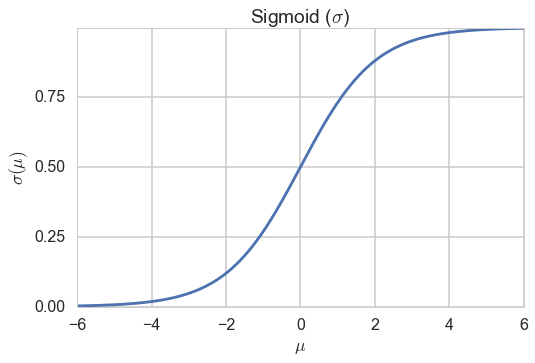
\includegraphics[scale=0.5]{sigmoid}
\end{figure*}


\noin The \textit{hypothesis}, $h_\theta(\boldx)$ given the weights $\theta$, is defined as
\begin{align*}
h_\theta(\boldx) &= \sigma(\theta^T\boldx) = \sigma \Big(\sum_{i=1}^n \theta_i \boldx_i \Big) \\ 
\Pr(y | \boldx, \theta) &= \Bern(y | h_\theta(\boldx))
\end{align*}

\noin Finally, $y$ is mapped to the discrete binary set $\{0, 1\}$ using a decision boundary $d$, where $0 \leq d \leq 1$.
\begin{align*}
h_\theta(\boldx) \geq d &\to y = 1 \\
h_\theta(\boldx) < d &\to y = 0 \\
\end{align*}

\noin Based on training data, a logistic regression model learns to optimize its predictions for newly observed data by updating the weights $\theta$. The weights in $\theta$ can be thought of as the control gates for the flow of information, and increasing the value of weight represents an increase in the importance of that information. In order to make the parameter update, a cost function $J$ is used to generate an error metric for the predicted outcome $h_\theta(\boldx)$ based on the "correct" observed outcome $\boldy$ for each observation-outcome pair in the training data. $\theta$ is then updated based on $J(\theta)$ by a method known as stochastic gradient descent (SGD). The ultimate objective, using SGD, is to minimize the cost $J(\theta)$ over the training data. 
$$J(\theta) = \frac{1}{m} \sum_{\boldx} Cost(h_\theta(\boldx), \boldy)$$
Therefore, the optimal parameters $\hat{\theta}$ are $$\hat{\theta} = \argmin_\theta J(\theta | \mathcal{X}, \mathcal{Y})$$

Multinomial logistic regression is a generalization of logistic regression to the case where we want to classify data into $K$ classes, not just two. The objective is to develop a hypothesis to estimate $\Pr(\boldy = k | \boldx)$ for $k \in 1, \ldots, K$. This is useful in handwritten digit recognition, for example, where $\boldx$ is a numerical representation of an image, and $h_\theta(\boldx)$ describes the probability that the image represents a specific digit for all digits 0-9 ($K=10$). $\argmax_k h_\theta(\boldx)$ therefore tells us which digit is most likely represented in the image. \\

In order to represent $K$ classes, $\theta$ is now a \textit{matrix} of weights, making $\theta^T\boldx$ an activation \textit{vector}. The sigmoid function is replaced with the softmax, which generalizes the sigmoid function and normalizes the activation vector such that the resulting vector represents a probability distribution over the $K$ classes. Since $h_\theta(x)$ is a distribution, its elements must sum to 1.\\

$$h_\theta(\boldx) = \begin{bmatrix}
			P(\boldy = 1| \boldx, \theta) \\
			P(\boldy = 2| \boldx, \theta) \\
			\vdots \\
			P(\boldy = K| \boldx, \theta) \\
			\end{bmatrix}
			= \frac{1}{\sum_{i=1}^K \exp(\theta^{(i)T}\boldx)}
			\cdot \begin{bmatrix}
			\exp(\theta^{(1)T}\boldx) \\
			\exp(\theta^{(2)T}\boldx) \\
			\vdots \\
			\exp(\theta^{(K)T}\boldx) \\
			\end{bmatrix}$$\\
			
\noin where $\theta$ is represented as

$$\theta = \begin{bmatrix} | && | && | && | \\
		\theta_1 && \theta_2 && \ldots && \theta_K \\ 
		 | && | && | && |
		\end{bmatrix}$$ \\

and the most likely classification is the class $k$ with the greatest probability given $\boldx$ and $\theta$
$$\argmax_k Pr(\boldy = k| \boldx, \theta)$$


\subsection*{Neural Networks}

In this section, we introduce \textit{artificial neural networks}, a family of machine learning models that are the primary models for this thesis. Neural networks give us a way to model deeper interactions, and to generate predictions based on a combination of many cascading, non-linear functions. They are exceptionally powerful, and by the Universal Approximation Theorem (Cybenko et. al. 1989), a feed-forward 3-layer neural network of finite size is proven to approximate any continuous function bounded by $n$ dimensions with any desired non-zero error \citep{goldberg2015nnlp}. As in multinomial logistic regression, the objective is $K$-class classification. Neural networks are loosely inspired by the architecture of biological neural networks, where the complex decisions computed by the human brain is a function of many, small computations made by individual neurons. In an artificial neural network, the "neuron" is a computational unit that accepts a vector input and returns a scalar output. Neurons are organized as a series of layers, where the first is referred to as the "input" layer, the intermediary layers being the "hidden" layer, and the final layer being the "output" layer. In order to obtain the $K$-class distribution, $\boldx$ is "fed forward" through the network by a process known as forward propagation. The process is shown below for a 3-layer network, where $\sigma$ is the sigmoid function (applied element wise). $\theta^{(i)}$ is the matrix of parameters that control the mapping of input units to hidden units for the $i$th layers. $\boldb^{(i)}$ is the bias neuron for the $i$th layer. $L_i$ is the size of the $i$th layer.
\begin{align*}
\boldz^{(1)} &= \theta^{(1)T}\boldx + \boldb^{(1)} \\
\bolda^{(1)} &= \sigma(\boldz^{(1)}) \\
\boldz^{(2)} &= \theta^{(2)T}\bolda^{(1)} + \boldb^{(2)} \\
\bolda^{(2)} &= \sigma(\boldz^{(2)}) \\
\boldz^{(2)} &= \theta^{(3)T} \bolda^{(2)} \\
h_{\theta}(\boldx) &= \sigma(\boldz^{(3)})
\end{align*}

where $$x \in \reals^m, h_{\theta}(\boldx) \in \reals^K, \theta^{(i)} \in \reals^{L_{i} \times L_{i+1}}, b^{(i)} \in \reals^{L_{i}}$$

When a layer is reached, each neuron in the layer performs a linear combination of the input and its parameters, applies a non-linear function (i.e. sigmoid $\sigma$), and then passes the result forward to each neuron in the next layer. Each connection between two neurons also carries a separate, adjustable parameter. This continues until the final layer, where the output layer returns a vector that is forwarded through a softmax function to obtain the $K$-dimensional distribution $h_{\theta}(\boldx)$.

\begin{figure*}[h]
\caption[Neural network representation]{Abstract representation of a 3-layer neural network architecture, where each circle represents a neuron. $\theta$ controls the flow of information between layers.}
\centering

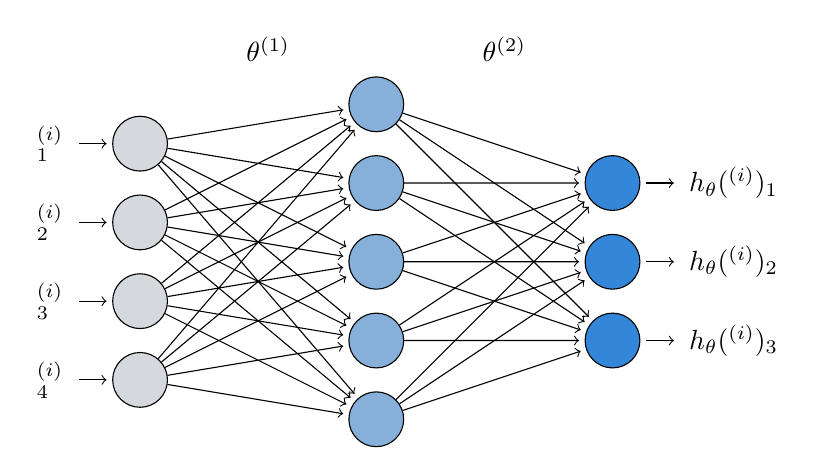
\begin{tikzpicture}[shorten >=2pt,->, draw=none, node distance=3cm]
    \definecolor{gray}{RGB}{213, 217, 222}
    \definecolor{lightblue}{RGB}{134, 176, 217}
    \definecolor{deepblue}{RGB}{52, 134, 217}
    \tikzstyle{every pin edge}=[<-,shorten <=2pt]
    \tikzstyle{neuron}=[draw, circle, inner sep=7pt]
    \tikzstyle{input neuron}=[neuron, fill=gray];
    \tikzstyle{output neuron}=[neuron, fill=deepblue];
    \tikzstyle{hidden neuron}=[neuron, fill=lightblue];
    \tikzstyle{annot} = [text width=4em, text centered]

    % Draw the input layer nodes
    \foreach \name / \y in {1,...,4}
    % This is the same as writing \foreach \name / \y in {1/1,2/2,3/3,4/4}
        \node[input neuron, pin=left: $\boldx^{(i)}_\y$] (I-\name) at (0,-\y) {};

    % Draw the hidden layer nodes
    \foreach \name / \y in {1,...,5}
        \path[yshift=0.5cm]
            node[hidden neuron] (H-\name) at (3cm,-\y cm) {};

    % Draw the output layer node
    \foreach \name / \y in {1,...,3}
    	 \path[yshift=-0.5cm]
		node[output neuron, pin={[pin edge={->}]right: $h_{\theta}(\boldx^{(i)})_{\y}$}] (O-\name) at (6cm,-\y cm) {};

    % Connect every node in the input layer with every node in the
    % hidden layer.
    \foreach \source in {1,...,4}
        \foreach \dest in {1,...,5}
            \path (I-\source) edge (H-\dest);

    % Connect every node in the hidden layer with the output layer
    \foreach \source in {1,...,5}
    	\foreach \dest in {1,...,3}
        		\path (H-\source) edge (O-\dest);

    % Annotate the layers
    \node[annot,above of=I-1, right=0.8cm, node distance=1.2cm] (t1) {$\theta^{(1)}$};
    \node[annot,right of=t1] (t2) {$\theta^{(2)}$};
    %\node[annot,left of=hl] {Input layer};
    %\node[annot,right of=hl] {Output layer};
\end{tikzpicture}
\end{figure*}

For all neural models used in this thesis, the objective is to minimize \textit{negative log likelihood}. Likelihood ($\mathcal{L}$) is a function of the parameters $\theta$ given a set of observations $\mathcal{X}$, and it is in fact equivalent to the probability of those observations given the parameters.
$$\mathcal{L}(\theta | \mathcal{X}) = P(\mathcal{X} | \theta)$$
For mathematical ease, log likelihood is used.
$$\log \mathcal{L} = \log \prod_{i=1}^{m} h(\boldx_i | \theta) = \sum_{i=1}^{m} h(\boldx_i | \theta)$$
And maximizing log likelihood is equivalent to minimizing negative likelihood.
$$\hat{\theta} = \argmax_{\theta} \sum_{i=1}^{m} h(\boldx_i | \theta) = \argmin_{\theta} \Big[- \sum_{i=1}^{m} h(\boldx_i | \theta)\Big]$$

The parameters $\theta$ are updated by calculating $J(\theta)$ and computing the partial derivatives (the "gradients") of $J(\theta)$ with respect to each of the parameters. 
$$\theta_{j} = \theta_{j} - \alpha \frac{\partial J(\theta)}{\partial \theta_j}$$
The partial derivatives of $J$, or the gradient vectors, describe the direction of \textit{steepest ascent} of $J(\theta)$. So by subtracting these gradients at each update, the network descends towards a minimization of $J$. The learning rate, $\alpha$, adds a multiplicative factor that controls the strength of each gradient update. This process of passing gradients through the network and updating $\theta$ is known as backwards propagation.



\subsection*{Recurrent neural networks (RNNs) and sequential data}

An important limitation of "vanilla" (meaning standard) neural networks, like the ones described in the previous section, is that they treat each input independently of all other inputs. In supervised learning tasks where the input data is in the form of \textit{sequences}, recurrent neural networks (RNNs) are an effective model because of their ability to "remember" features of recent computations. Formally, a sequence of data is defined as a series of input vectors over a discrete set of time-steps, such that $\boldx_i$ is the input vector at time step $i$. RNN architecture is optimized for sequences of inputs and outputs, and they can train very effectively on datasets even when the inputs lack a naturally sequential order (\cite{karpathy2015rnn}).\\

At each time step, the recurrent model receives two inputs, the feature vector $x_t$ as well as the output of the hidden layer from the previous time step $s_{t}$. During forward propagation, an RNN internally stores the output of each hidden layer and returns a distribution for the next time step, $h_{t+1}$. The most basic RNN architecture, known as the Elman network or simple RNN (S-RNN) \citep[p.~56]{goldberg2015nnlp}, can be modeled as follows:
\begin{align*}
\bolda_i(\boldx) &= \sigma(\theta^{(1)T}\boldx_i + \theta^{(2)T}\boldy(\boldx_{i-1})) \\
\boldy(\boldx_i) &= g(\bolda_i(\boldx))
\end{align*}
where $$\theta^{(1)} \in \reals^{|\boldx| \times h}, \theta^{(2)} \in \reals^{h \times h}$$

\noin and $g$ is a non-linear transformation, such sigmoid ($\sigma$) or tanh. Note that the parameters $\theta$ can be updated in the middle of forward propagation over a sequence, or after the entire sequence has been fed through. Training an RNN follows the same procedure as standard neural networks - create a computation graph over time, calculate error for the most recent prediction, and then backpropagate the error across the unfolded network, generating gradients and updating the weights in $\theta$ \citep[p.~63]{goldberg2015nnlp}. \\

\begin{figure*}[h]
\centering
\caption[Recurrent neural network representation]{Abstraction of an RNN over a time series. The activation of the neurons in the hidden layer is a function from the previous layer (in this architecture, this is always the input layer) and the hidden layer output from the previous time step. }
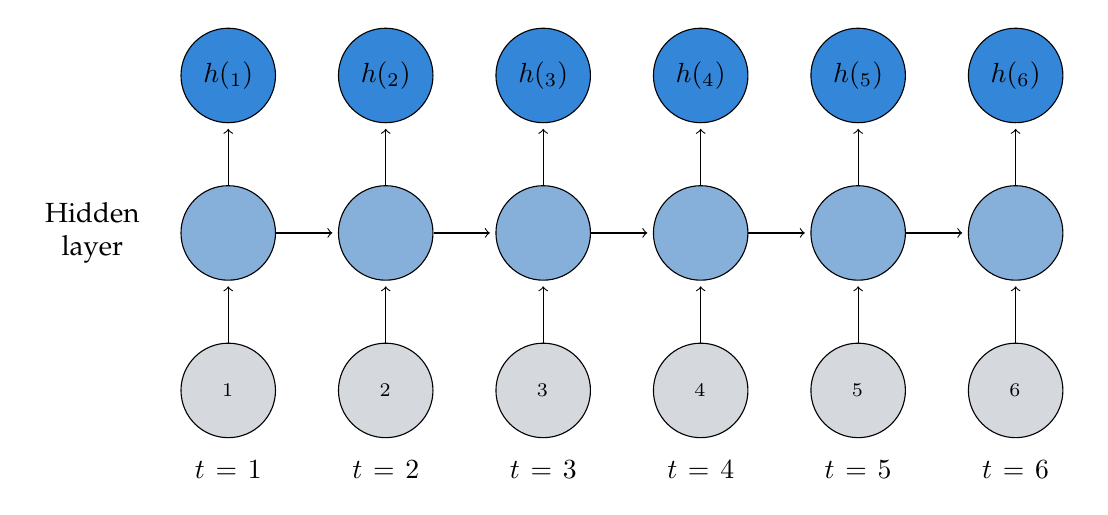
\begin{tikzpicture}[shorten >=2pt,->, draw=none, node distance=3cm]
    \definecolor{gray}{RGB}{213, 217, 222}
    \definecolor{lightblue}{RGB}{134, 176, 217}
    \definecolor{deepblue}{RGB}{52, 134, 217}
    \tikzstyle{every pin edge}=[<-,shorten <=2pt, thin]
    \tikzstyle{neuron}=[draw, circle, minimum size=12mm]
    \tikzstyle{input neuron}=[neuron, fill=gray];
    \tikzstyle{output neuron}=[neuron, fill=deepblue];
    \tikzstyle{hidden neuron}=[neuron, fill=lightblue];
    \tikzstyle{annot} = [text width=4em, text centered]

    \def\layerdist{2}
    % Draw the input layer nodes
    \foreach \name / \y in {1,...,6}
        \node[input neuron] (I-\name) at (\y * 2, \layerdist * 0) {$\boldx_{\y}$};
    \foreach \name / \y in {1,...,6}
    	\node[annot,below of=I-\name, node distance=1cm] (t1) {$t=\y$};

    % Draw the hidden layer nodes
    \foreach \name / \y in {1,...,6}
    	\node[hidden neuron] (H-\name) at (\y * 2, \layerdist * 1) {};

    % Draw the output layer node
    \foreach \name / \y in {1,...,6}
    	\node[output neuron] (O-\name) at (\y * 2, \layerdist * 2) {$h(\boldx_{\y})$};

    % Connect the input layer with the hidden layer
    \foreach \unit in {1,...,6}
    	\path (I-\unit) edge (H-\unit);
    
    % Connect the hidden layer with the output layer
    \foreach \unit in {1,...,6}
    	\path (H-\unit) edge (O-\unit);

    % Connect the recurrent layer
    \path (H-1) edge (H-2);
    \path (H-2) edge (H-3);
    \path (H-3) edge (H-4);
    \path (H-4) edge (H-5);
    \path (H-5) edge (H-6);

    % Annotate the layers
    \node[annot,left of=H-1, left=0.1cm, node distance=0.8cm] (t1) {Hidden layer};
\end{tikzpicture}
\end{figure*}

The recurrent model of incorporating feedback from the computation at the previous time step is a promising approach for the harmonization task, where the chorale can be represented as a sequence of melody notes with corresponding, interrelated harmonizations. \cite{karpathy2015rnn} famously cited the "unreasonable effectiveness" of recurrent neural networks in learning sequential data for a variety of tasks, including speech recognition, language translation, and image captioning. As a result, we hypothesize that recurrent models will perform particularly well on musical tasks that require contextualized decision-making and benefit from correlating temporally distant inputs.

\subsection*{Improving the recurrent model: Long Short-Term Memory networks}

Long Short-Term Memory networks (LSTMs) are a variant of RNNs that replace the hidden layer neurons with specialized cells for enhanced memory capabilities, first introduced by Schmidhuber and Hochreiter in 1997. In the original RNN architecture, the feedback is "short-term" in that $s_t$ is only a function of the input at time $t-1$ (and much more weakly for previous time steps). Therefore as the sequence is fed through the network, the signal from earlier time steps is gradually lost. This phenomenon is known as the "vanishing gradients problem" \citep[p.~56]{goldberg2015nnlp} and it constitutes a major drawback to using the original RNN architecture. LSTMs solve this long-term dependency issue by substituting the regular neuron with a \textit{memory cell} that can retain much more distant signals from previous inputs. Information is stored and segregated within the cell by use of multiplicative gate units, such as input, forget, and output gates. These gates allow information to flow through the cell without affecting other memory contents, while also deciding what cell  information should be kept versus overwritten by newer signals. A gate $\boldg$ is represented as a $n$-dimensional one-hot vector, and the values of $\boldg$ are considered parameters of the model. A value of 1 in a gate has the effect of retaining its corresponding signal element, while a value of 0 effectively eliminates that element. The deeper mathematical foundations for LSTMs are not necessary to understand, but they have proven to be exceptionally effective models, designed specifically for retaining information over long periods of time. When applied to music, LSTMs have proven effective at learning global musical structures and generating melodies (\cite{eck2002blues}; \cite{johnson2015compose}).

\begin{figure*}[h]
\centering
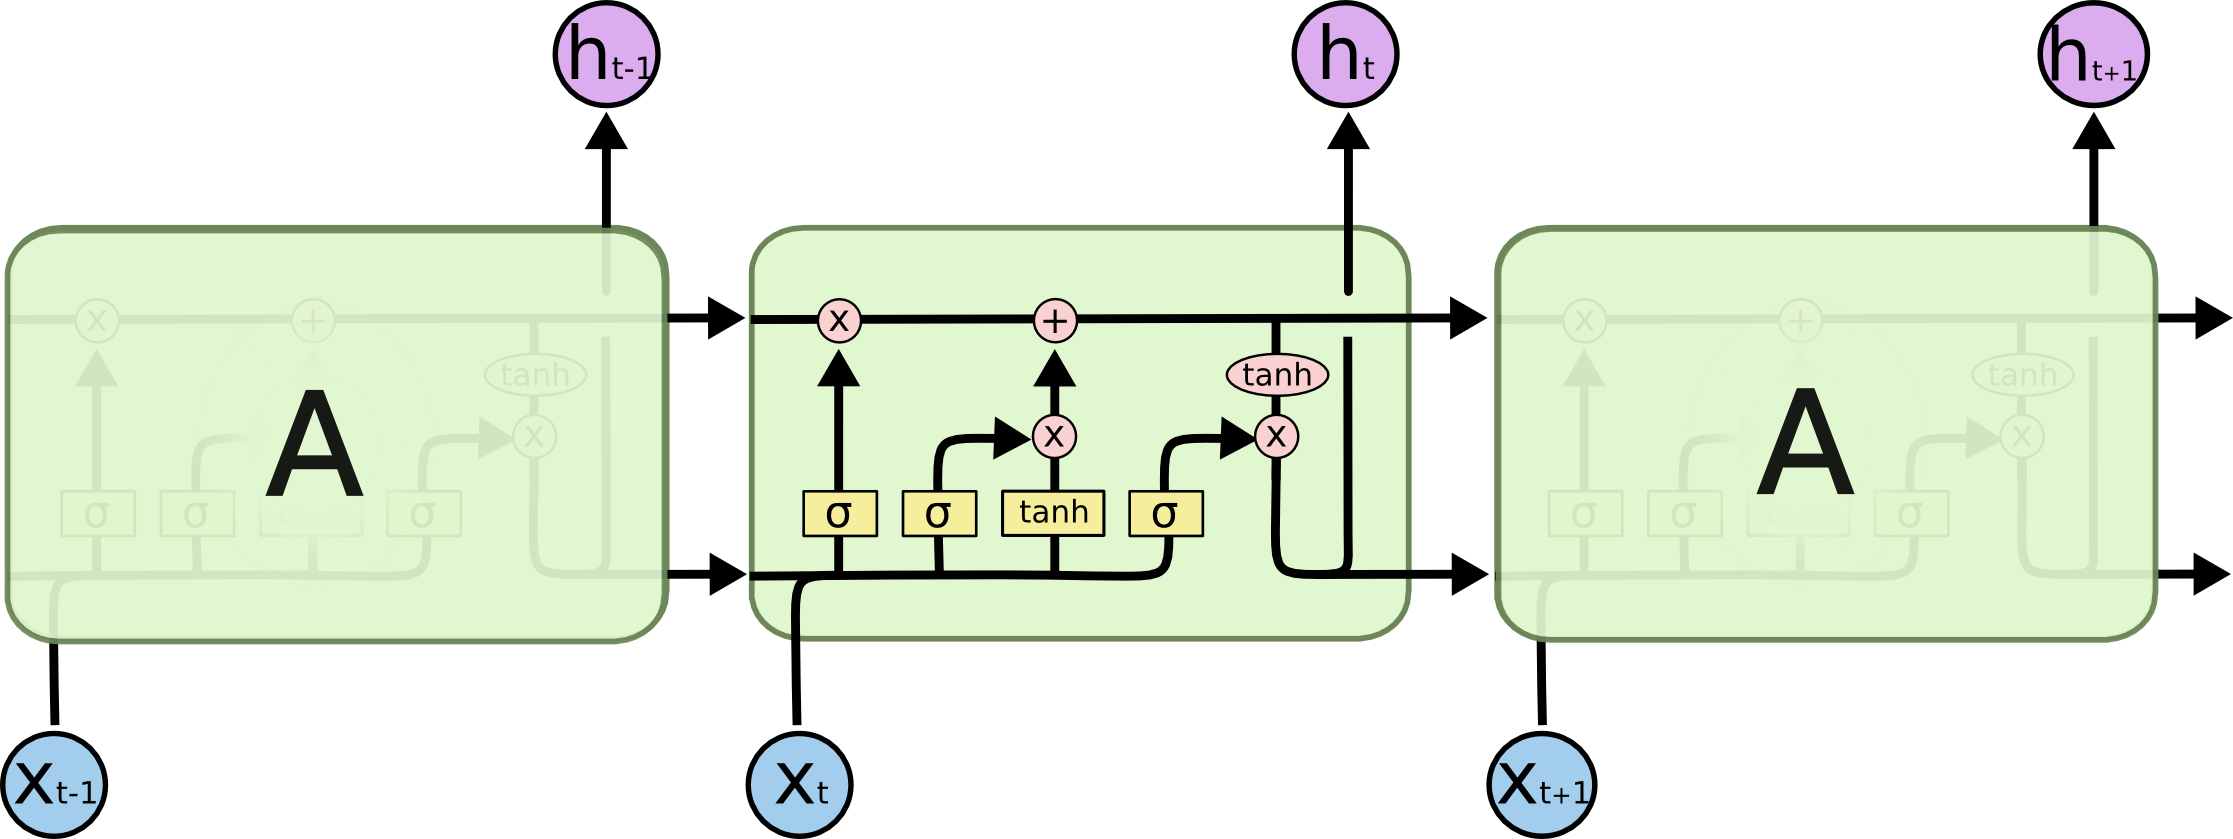
\includegraphics[scale=0.5]{lstm2}
\caption[LSTM memory cell]{The chained structure of an LSTM memory cell. Each cell contains multiple network layers, where the RNN presented previously has only one (the sigmoid layer). Diagram created by \citet{colah2015lstms}.}
\end{figure*}



%%%%%%%%%%
%-----------------------
%%%%%%%%%%

\section{Introducing tonal harmony and the Chorales}

The primary objective of this thesis is to train a variety of models on the four-voice chorales composed by J.S. Bach in order to learn the task of chorale harmonization. However, each model is not given an actual musical score as input, but rather a numerical representation of "features" extracted from the score. Features are variables that describe some aspect of the data, and a thoughtful selection of features is one of the largest factors that contributes to an effective model. The features selected from the chorales include both score-wide features, such as the key signature, as well as local features that describe the melody at a specific moment in numerical terms, such as the beat strength of the melody note. In order to understand the meaning of the musical features selected from the chorales and their significance in learning the task of harmonization, a tailored overview of tonal harmony and the properties of the chorales is provided here. Musical properties are described as computational objects to illustrate the ability to translate between these properties and numerical representation. \\

\subsection*{Pitch class, pitch, note}

The fundamental musical object in Western tonal music is the \textit{pitch class}. The tonal system operates over a series of 12 \textit{pitch classes}, and some pitch classes (i.e. C$\sharp$/D$\flat$) are referred to by different names depending on the current context. A pitch class is defined by its unique index - a integer between 1 and 12. It is common to assign the tonic pitch class as 1, the pitch class above it as 2, and so on.

\begin{center}
C, C$\sharp$/D$\flat$, D, D$\sharp$/E$\flat$, E, F, F$\sharp$/G$\flat$, G, G$\sharp$/A$\flat$, A, A$\sharp$/B$\flat$, B
\end{center}

A \textit{pitch} is an object defined by a pitch class and an octave, identifying a unique frequency. A common representation of pitch is MIDI (Musical Instrument Digital Interface) notation, which today remains the most widely used protocol for communication of musical information between electronic instruments. In MIDI, a pitch is identified by a unique integer between 21 and 108 (inclusive). However, a disadvantage to MIDI is that it conflates enharmonic pitches (i.e. C$\sharp$5 has the same MIDI value as D$\flat$5), so information about the function of a pitch within a key signature is lost with this representation. \\

We then define a \textit{note} as a pitch with the additional feature of duration.

\subsection*{Scale, chord, key}

The musical objects defined here are fundamental indicators of harmonic information. A \textit{scale} is an ordered collection of pitch classes defined by an initial pitch class and a quality - major or minor - that defines the intervals between each note in the collection. Each pitch class in the scale is given an indexed scale degree and a name. The two most important elements in the scale are the "tonic" ($\hat{1}$) and "dominant" ($\hat{5}$). But more generally, a melody over a scale is guided by the characteristic tension or stability of the scale's pitch classes. The "tonic" represents the ultimate point of stability, whereas the leading tone ($\hat{7}$) creates a sense of motion towards the tonic. Therefore, pitch is a crucial feature in predicting the continuation of a melody or the harmonization of an existing melody. \\

The strong parallel between scales and chords can be defined as a \textit{chord-scale duality}. A \textit{chord} is a collection of three or more notes sounded together. The pitches that comprise a chord imply a scale that contains those pitches; and similarly, a scale implies the set of \textit{triads} that can be constructed starting from each note of the scale. The important connection is that both scales and chords express harmonies through the pitch classes that comprise them.\\

\begin{figure*}[h]
\centering
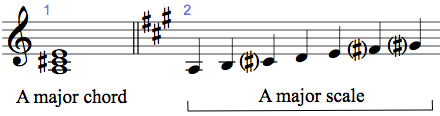
\includegraphics[scale=0.6]{chord-scale}
\caption{Chord-scale duality}
\end{figure*}

The \textit{key} of a piece is a combination of two pieces of harmonic information - the tonic pitch class, and the chord (or scale) that represents full harmonic resolution. In major and minor keys, this chord is a \textit{triad}, which in the key of C major is the pitch class set \{C, E, G\}. The triad alone is able to define the diatonic scale for the piece, which is represented symbolically as a key signature that specifies the pitch classes of the diatonic scale.


\subsection*{Harmonic analysis and motion}

When harmonizing a chorale, an important first step is to analyze the chorale melody and determine the chord progression that the harmonizing voices will describe. A standard approach for notating chord progressions in classical harmony is Roman numeral analysis. Roman numeral analysis describes a harmony by assigning a Roman numeral based on the chord root and a uppercase or lowercase version (i.e. \rom{2} vs. \lrom{2}) based on the chord quality. Superscripts are used to denote chord inversions, indicating which pitch class in the chord appears in the lowest voice \citep[pg.~68-9]{laitz2008}. For example, in the key of A major, the A major triad \{A, C$\sharp$, E\} is assigned \rom{1} and an E dominant 7th chord \{E, G$\sharp$, B, D\} is assigned \rom{5}$^7$ based on the E major triad, notated as \rom{5}, and a seventh extension that creates the dominant quality. Roman numeral analysis is powerful because it focuses on the harmonic information stored in triads. The motion between tonic and dominant triads alone can firmly establish a key, as well as a sense of tension and resolution that is generated by harmonic motion away from and towards the tonic harmony \citep[pg.~106]{laitz2008}. \\

Importantely, context is a crucial factor in performing Roman numeral analysis because each harmony is analyzed with respect to the key of the chorale as well as the harmonies that preceded it. This is why harmonies are often described as a progression, or a \textit{sequence}. The ordering of harmonies - like the ordering of words in a sentence - is a essential feature of the progression, and an important feature to consider when constructing models to generate new progressions. \\

\textit{Cadences} are the components of a harmonic progression that conclude a musical phrase or section. They are important harmonic indicators that lead to a point of a resolution or heightened tension, depending on the type of cadence, and as a result they control the flow of the music. Statistically, the ability of a model to accurately predict the location and quality of a cadence can serve a useful qualitative indicator of a model's performance because cadences are the most defining feature of a harmonic progression. \\


\subsection*{Bach's settings of the chorales}

A \textit{chorale} is a congregational hymn that first came into use during the early decades of the German Protestant Reformation, under Martin Luther. These hymns were originally composed as a one-voice melody with lyrical text, and composers of the time drew heavily (and sometimes borrowed verbatim) from existing secular songs, medieval Gregorian chant, and other sacred works when writing new chorales. In the Baroque era, the composer Johann Sebastian Bach revived the chorale tradition and composed several new chorale melodies. However, his most lasting contribution to the chorale form remains his hundreds of chorale harmonizations, which were inserted into many of his larger vocal and instrumental compositions, including the St. Matthew Passion and the cantatas \citep{leaverchorale}. His harmonization of four-voice chorales - of which 341 exist in the Riemenschneider collection - are masterful studies in four-voice counterpoint, and they remain a guide for modern church musicians, jazz writers, arrangers and students alike. This corpus established fundamental conventions for tonal harmony with respect to voice leading, cadential movement, and intervallic relationships between voices. \\

Structurally, the chorale is written for the four standard voice ranges: soprano, alto, tenor, and bass. The original chorale melody is sung by the soprano, while the lower voices collectively embody the \textit{harmonization} of the melody. It closely resembles the chordal motion of the modern sacred hymn, and the rhythmic complexity of the chorales is intentionally minimal in order to draw focus to the harmonic motion taking place on each beat. The entire chorale is segmented into shorter phrases by a series of \textit{fermatas} that indicate pauses and points of emphasis. In the Chorales, fermatas denote the conclusion of cadences, where a tension or resolution is firmly established. \\

In order to full understand the chorale form, it must be viewed in multiple dimensions. In the vertical dimension, the notes of each voice at time $t$ can be heard simultaneously as a chord; and therefore, the chorale can be abstracted to a four-voice chordal progression. Learning to recognize and generate choral progressions is the primary task of this thesis. The progression is guided by the cadences that structure each phrase, and each cadence is defined by the relationship between the melody and the bass line. The inner voices (alto and tenor) function as supportive voices that "fill out" the harmonies. In the linear dimension, the chorale represents a combination of four independent but complimentary melodic lines, where the contour of each line is governed by the conventions of \textit{voice leading}. Voice leading embodies a broad set of characteristics, but they include rules about preferred and undesired intervals, parallel and contrary motion, and the use of passing tones for creating smooth melodic lines. The conventions of voice leading the acceptable motion in each voice as the harmony shifts in the vertical dimension. \\

\begin{figure*}[h]
\caption[\textit{Nun lob mein' Seel', den Herren}, harmonized by J.S. Bach]{Opening phrase of the chorale \textit{Nun lob mein' Seel', den Herren}, harmonized by J.S. Bach.}
\centerline{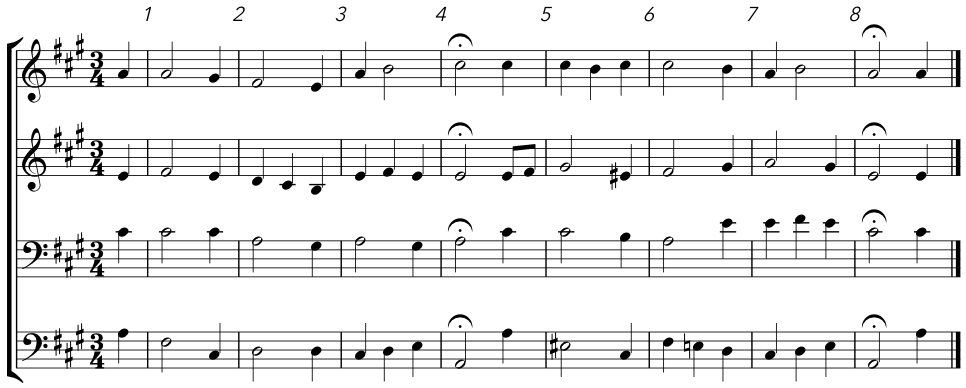
\includegraphics[scale=0.45]{chorale_mine}}
\end{figure*}
\clearpage
The opening section of the chorale \textit{Nun lob mein' Seel', den Herren} (Figure 1.6) illustrates the importance of \textit{context} in chorale harmonization. Bach's choice of harmonization for each beat is not an independent decision, but rather a choice guided by the harmonic destination of each phrase, which the composer almost certainly decided in advance of writing out the other voices. The harmony at time $t$ constrains the set of harmonies that it can smoothly transition to at time $t+1$. Consequently, the reverse is true: if we decide to assign a certain harmony at time $t$, the preceding harmonies must be chosen with the constraint that they provide a satisfying towards that harmony. Note, for example, the \lrom{2}$^6$ - \rom{5} - \rom{1} cadences that Bach constructs in measures 3-4 and 7-8 of Figure 1.6. Were we harmonizing this chorale ourselves and decided to assign a \lrom{2}$^6$ harmony to beat 2 of measure 3 or 7, we would constrain which harmonies we could convincingly transition to on beat 3. The fermata on the downbeat of measure adds the additional constraint that a cadence - likely an authentic (\rom{1}) or half (\rom{5}) cadence - concludes on that beat. The harmonization of beat 3 must therefore bridge its surrounding harmonies to satisfy the expression \lrom{2}$^6$ - * - \{\rom{1}, \rom{5}\}. \\ 

The C$\sharp^7$ harmony in measure 5 further illustrates the need for careful planning when constructing a harmonic progression because the C$\sharp^7$ harmony isn't diatonic in the chorale's key of A-major. Non-diatonic harmonies most commonly occur in areas of tonicization - when the harmony briefly establishes a new tonic - or when the harmony is functioning a secondary dominant. In this instance, the C$\sharp^7$ is functioning as a secondary dominant, since it acts a dominant harmony with respect to $F\sharp$-minor in measure 6. Secondary dominants are an effective tool for prolonging the resolution towards a certain harmony, and Bach uses them frequently to expand his harmonic palette. The chorale \textit{Warum betr�bst du dich, mein Herz} (Figure 1.7) also contains non-diatonic harmonies functioning as secondary dominants, which facilitate the chromatically ascending bass line in measures 2 and 3.
\clearpage

\begin{figure*}[h]
\caption[\textit{Warum betr�bst du dich, mein Herz}, Roman numeral analysis]{ Roman numeral analysis of \textit{Warum betr�bst du dich, mein Herz} }
\centerline{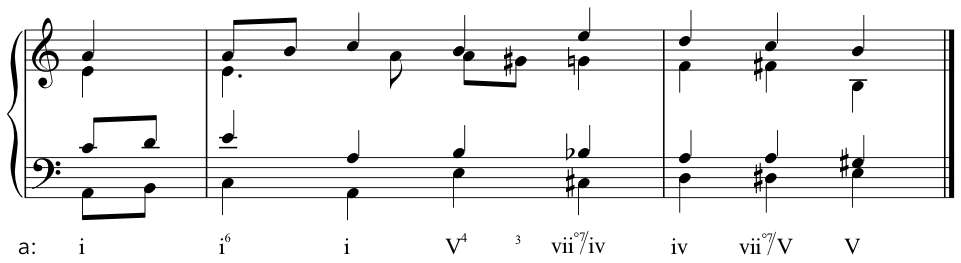
\includegraphics[scale=0.45]{chorale2_mine}}
\end{figure*}

In summary, the process of harmonization requires consideration of the larger harmonic structure and how each chosen harmony will contribute to the harmonic progression of the phrase. Characteristics of the melody note - such as pitch, beat strength, or the presence of a fermata - provide information about what harmonies might compliment it, while knowing the location of the next fermata or the preceding harmony inform how future harmonies should be chosen to create a satisfying progression. \\



%%%%%%%%%%%%%%%%%%
% CHAPTER 2
%%%%%%%%%%%%%%%%%%


\chapter{Establishing a baseline model}

\section{Motivation for the harmonization task}

J.S. Bach's collection of chorale harmonizations is used as the dataset for this thesis because it remains one of the largest and finest examples of four-part counterpoint in Western music. Each harmonization is a complex solution, satisfying a variety of voice leading and cadential constraints, as well as innumerable other conventions of musical style. Chorale harmonization is therefore a fundamentally difficult computational task. The reader might ask whether a rule-based approach is suitable to this task. Couldn't musical constraints would be computationally encoded and then only harmonizations that satisfy them are generated? However, a purely rule-based approach is rendered impractical by a couple important factors. One is the sheer number of conventions that would need to be encoded, each with a varying level of specificity and precedence with respect to the other encoded conventions. Determining precisely what those conventions are is an even more difficult problem, since many chorale constraints are vaguely defined or flexible in application. Another reason for avoiding a rule-based approach is that many different harmonizations exist that satisfy a given chorale melody. The goal is not to simply produce satisfying harmonizations, but to \textit{approximate} Bach's style of harmonization as closely as possible. Unlike a rule-based model, an \textit{adaptive} model updates its parameters to capture the complex correlations and patterns it discovers in the training set of harmonizations. Applying those parameters to a new chorale melody will then yield a predicted harmonization, and its predictions will directly reflect (and only reflect) the harmonizations the model was trained upon.
  
\section{Literature review}

\citet{hild1992harmonet} presented the first effective neural network approach for harmonizing chorales. Referring to their model as HARMONET, their prediction harmonizations were qualitatively described to on the level of an "improvising organist" (p. 272), although little quantitative evidence is provided. The task decomposed into three subtasks, each learned by a neural network. A harmonic skeleton is first created by sweeping through the chorale melody and determining a harmony for each beat, where the harmony is represented by a unique figured bass notation. For each time step $t$, the network takes an input a window of information, including the harmonies chosen in the interval$[t-3, t-1]$ and the melody pitches in the interval $[t-1, t+1]$. The resulting harmonic skeleton is passed to another network to generate a chord skeleton, which selects the inner voices based on the input figured bass, and a final network adds ornamental eighth notes to restore passing tones between chords. Although, HARMONET demonstrated strong success at harmonizing melodies, the model used external "chorale constraints" \citep[p.~271]{hild1992harmonet} in constructing the chord skeleton in order to avoid unfavorable chord structures. The models presented in this paper attempt to learn the task of harmonization without any such form of manual intervention in the network's learning process. \\

Substantial work has been done in the field of music generation using RNNs and LSTMs that demonstrate their ability to learn complicated musical structures and relate temporally distant events, particularly in the realm of melodic generation. \citet{petri1995bebop} developed a neural network that generates a jazz bebop melody over series of chord changes. The network achieves melodic continuity by using a "target-note technique", where the end of a previous melody segment and the present chord are used to predict the next melodic pattern at time $t+1$, while the following chord at time $t+2$ is use to optimize of the melodic pattern, thereby smoothing the melodic transitions over chord changes. \citet{eck2002structure} improved on the results of \citet{mozer1994neural}, who used RNNs to compose melodies with chordal accompaniment but found the resulting music lacked larger thematic and phrase structure. They attributed Mozer's results to the "vanishing gradients" problem (described briefly in chapter 1) and then trained LSTMs to first generate the chordal structure and use that as a input to the LSTMs that generates a blues-style melody with promising results. \citet{franklin2006jazz} also used LSTMs to compose jazz melodies over a chord progression, training the networks on a dataset of well-known jazz standard melodies. \\

Research specifically on modeling the Bach chorales has seen a variety of approaches. Many of these studies have been based on a dataset generated by \citet{allan2005harmonising}, which contains hundreds of chorales transposed to C major or C minor and then sampled every quarter note. The dataset contains the pitches (encoded as MIDI values) for all voices at each time step of a chorale. \citet{allan2005harmonising} trained Hidden Markov Models (HMMs) on the data to model chorale harmonization, creating a probabilistic framework for deciding the most likely choice of alto, tenor, and bass notes to complement the melody in each time frame. More recent work has focused on music \textit{generation} models rather than completive models. \citet{boulanger2012modeling} used this version of the dataset, along with multiple other corpuses, to make a comprehensive survey of music generation models that performed next-step prediction for \textit{all} voices. Using log-likelihood and overall accuracy as the performance metrics on test data, a specific flavor of RNNs was found to be most effective on all corpuses used in the study. Other studies have sought to "re-construct" chorales using more sophisticated neural models, including a large-scale survey of polyphonic music modeling that evaluated the performance of eight LSTM variants \citet{greff2015lstm}. Both previous papers mentioned highlight the use of RNNs and LSTMs as effective models because of their ability to learn temporal dependencies within polyphonic music (i.e. how distant musical events can be related). Notably, the latter found the "vanilla", unmodified LSTM equally effective as the other variants \citep[p.~7]{greff2015lstm}, which is why the standard neural network architecture is incorporated into the neural models for our research. \\

Our approach consists of applying a variety of non-neural and neural models to the task of chorale harmonization. Recent harmonization and generative models (\cite{allan2005harmonising}; \cite{kaliakatsos2014}; \cite{greff2015lstm}) relied on a dataset that includes only pitch information about each time step, and the objective was in all cases next step pitch prediction. Our goal is to extract a new set of features from Bach's chorales and examine how those features improved or worsened model performance. Moreover, the objective is to learn a series of musical processes that decide the harmony at each time step that include both harmonic analysis and note selection. We chose this approach to mimic the decisions a musician would make today in harmonizing a chorale.

\section{Baseline models}

Due to the unique classification problems examined in this thesis, previous computational research on the chorales does not provide any adequate baseline models. Baseline models are important because they provide a basis for comparison when evaluating more sophisticated model architectures. As the complexity of the model changes and features are added or removed, it is important a baseline performance metric to compare against and see how changes to the model improved or worsened the results. In classification problems, a simple baseline model to consider is one that chooses the most common class for every observation. We refer to this as the Most Common Class Frequency (MCCF) baseline model. Three other classifiers are used to get a comprehensive set of baseline performances upon which we can judge the complexity of different harmonization tasks. These classifiers are described below: \\

\textit{Multiclass logistic regression} was introduced in Chapter 1 as a generalization of the binary classification system of logistic regression. Despite its name, this regression is a linear model. The objective is to minimize the following cost function, given the learned parameters $\theta$.
$$ J(\theta) = -\frac{1}{m} \sum_{i = 1}^{m} \sum_{k  = 1}^{K} \{ \boldy^{(i)} = k \} \log \Big( \frac{ \exp(a_{ik}) } { \sum_j \exp(a_{ij}) } \Big) $$
Where $m$ is the number of examples, $k$ is the number of classes, and $a_{ik}$ is the "activation" function $\theta^{(k)T} x^{(i)}$, denoted for the $i$th example and the $k$th class. \\

\textit{Multinomial naive Bayes} generalizes the naive Bayes algorithm for multi-class data, and it makes the "naive" assumption of independence between every pair of input features. The assumption therefore states that, given the input vector $\boldx$ and the class $c \in [1, K]$
$$P(\boldx | c) = P(\boldx_1, \boldx_2, \ldots, \boldx_n | c) = \prod_{i=1}^{n} P(\boldx_i | c)$$
And based on that assumption, this baseline classifier the predicted output class is decided by
$$P(c | \boldx) = \frac{ P(\boldx | c) P(c) }{ \sum_j P(\boldx | C_j) P(C_j) } = \frac{ \prod_i P(\boldx_i | c) P(c) }{ \sum_j \prod_i P(\boldx_i | C_j) P(C_j) }$$

\textit{Random Forest} is a powerful supervised learning technique that involves classification based on a majority vote of a series of small decision trees. Each tree is initialized with data from a random subset of features and is then trained on the data by sampling inputs with replacement. The randomness involved in this technique is known to be highly effective in preventing overfitting on training data, and it generalizes well on weaker datasets where one or more training examples do not strongly suggest differences between classes \citep[p.~18]{breiman2001}.


\section{Harmonization tasks}

Each model was tasked with learning both harmonic analysis and harmonic prediction processes. Each of these processes is referred to as a \textit{subtask}, and together they represent a full set of decisions about the harmony for a specific time step. Initially, 4 subtasks were selected. The first two are referred to as harmonic analysis subtasks because they relate to the general classification of harmony.
\begin{enumerate}
\item \textit{Roman numeral}. This subtask symbolizes the selection of the numeral in Roman numeral analysis. The numeral carries most of the weight in harmonic classification since it implies the both the root of the harmony as well as the quality of the triad built upon it (i.e. major, minor, diminished, etc.).
\item \textit{Inversion}. This subtask decides the chord inversion, which provides additional harmonic information about the ordering of the voices. The inversion implies which pitch class in the harmony is assigned to the bass voice, so this is also in some sense a harmonic \textit{prediction} subtask as well. However, it is designated as analytical because the inversion is primarily a component of Roman numeral analysis. Functionally, an inverted harmony carries implications for future harmonies. First inversion triads can lessen the weight of a tonic or dominant harmony by not placing the chord root in the bass. Inversions are also utilized to improve voice leading bass.
\end{enumerate}
The next two subtasks are referred to as harmonic prediction subtasks, as they decide which pitches are assigned to the inner voices (alto and tenor).
\begin{enumerate}
\setcounter{enumi}{2}
\item \textit{Alto}. This subtask decides which pitch should be assigned to the alto voice, which should be a pitch that supports the chosen harmony. 
\item \textit{Tenor}. This subtask decides the pitch assigned to the tenor voice. Selection of the tenor voice completes the harmonization.
\end{enumerate}

\subsection{GCT encoding}

While Roman numeral analysis has been the traditional method for describing harmony in the Chorales, it presents issues for statistical learning. Roman numeral classification mainly depends on the key signature, but also requires the context of the preceding harmonies. For example, a D major chord in a C major chorale might be labelled as a \rom{2} or \rom{5}/\rom{5} depending on whether a modulation to D major had occurred or whether the preceding harmonies indicate that it functions as a secondary dominant. During training, finding two or more inputs that suggest a D major chord but are labeled differently can cause confusion in learning, particularly since in non-recurrent models there is no sense of context about other local harmonies. Roman numeral chord labeling can be further complicated by the presence of non-chord tones, which makes, for example, differentiating \rom{4}$^6$ and \lrom{2}$^7$ chords computationally confusing.\\

The general chord type (GCT) representation provides an idiom-independent solution to encoding harmony that assigns a unique encoding to each chord, regardless of context \citep{2014gct}. To encode a chordal harmony, the GCT algorithm takes as input the chord to be encoded, a pitch scale that describes the tonality, and a binary "consonance vector" $\boldv$ such that $\boldv[n] = 1$ if an interval of $n$ semitones is considered consonant for $0 \leq n \leq 11$. In this study, I chose $\boldv = [1, 0, 0, 1, 1, 1, 0, 1, 1, 1, 0, 0]$.  GCT then constructs an ordering of the chord pitches that maximizes the consonant intervals between all pairs of pitches. The remaining notes that create dissonant intervals are labeled as "extensions". Finally, the algorithm outputs an encoding of the form [root, [base, extensions]], where root is the pitch class of the chord root relative to the tonic, and the base is the ordering of maximal consonance. I adapted the algorithm to also output the degree of inversion, where 0 represents root position, 1 represents first inversion, and so on. Figure 2.1 demonstrates an application of the GCT algorithm to a tonal harmonic progression, comparing the Roman numeral analysis with the GCT encoding. The base [0, 4, 7] encodes a major triad, while [0, 3, 7, 10] encodes a minor seventh chord. \\

\begin{figure}[h]
\begin{center}
\caption[GCT vs. Roman numeral harmonic encoding]{Comparison of GCT and Roman numeral analysis notation, courtesy of \citet{2015gct}.}
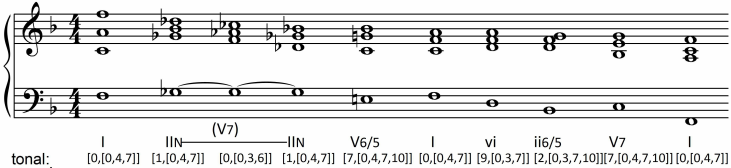
\includegraphics[scale=0.54]{images/GCT}
\end{center}
\end{figure}

In comparison with a Roman numeral analysis dataset compiled by David Temperley, GCT labeled 92\% of the chords accurately, of which about 1/3 of mislabeled chords were diminished sevenths - excusable because each note in the chord can function as the root \citep[p.~3]{2015gct}. In order to minimize duplicate encodings, I implemented the following policies, partially drawn from suggestions by the original authors of GCT encoding.
\begin{enumerate}
\item For dyads, prefer an interval of a 5th over a 4th, and an interval of a 7th over a 2nd.
\item Preference encodings where all intervals are larger than a major 2nd. This heuristic preferences a minor 7th or a major chord with an added 6th, and generally more evenly spaced encodings.
\item If more than one encoding remains, choose randomly.
\end{enumerate}

The GCT algorithm was incorporated into a newly generated dataset for the chorales by replacing the numeral and inversion subtasks in $\boldY$ with the new root, base, and inversion subtasks. The root subtask establishes the chord root, while the rest of the chord structure is determined by the base. As in Roman numeral analysis, the inversion implies which chord tone is assigned to the bass. As well, the new dataset classifies the tenor and alto voices by their distance from the tonic pitch, instead of as encoding MIDI values directly, in order to make all subtasks key-independent and reduce the output class space to a maximum of 12 classes (for the 12 chromatic intervals).\\

The same baseline models were used to evaluate the new subtasks. In both cases, there were 293 chorales in the training set, and 33 chorales in the test set.

\subsection{Defining harmonization subtasks}

\noin Mathematically, the objective is approximate the complex function $f: \boldX \to \boldY$
\begin{itemize}
\item $\boldX \in V^{n \times m}$ is the aggregate input data over $n$ observations, each with $m$ features ($\boldx \in \reals^m$)
\item $\boldY \in Y^{n \times K}$ contains the output distributions for a subtask over $n$ observations and $K$ output classes
\end{itemize}
Each observation describes the melody note at a specific time step, which we use to predict the most probable harmony and voicing for that time step as a series of smaller subtasks.  Figure 1 illustrates the subtask learning process.

\begin{figure}[h]
\begin{center}
\caption[Harmonization subtask model]{Harmonic subtasks: collectively, they describe the harmony for a specific time step and which pitches are assigned to the alto, tenor, and bass voices.}
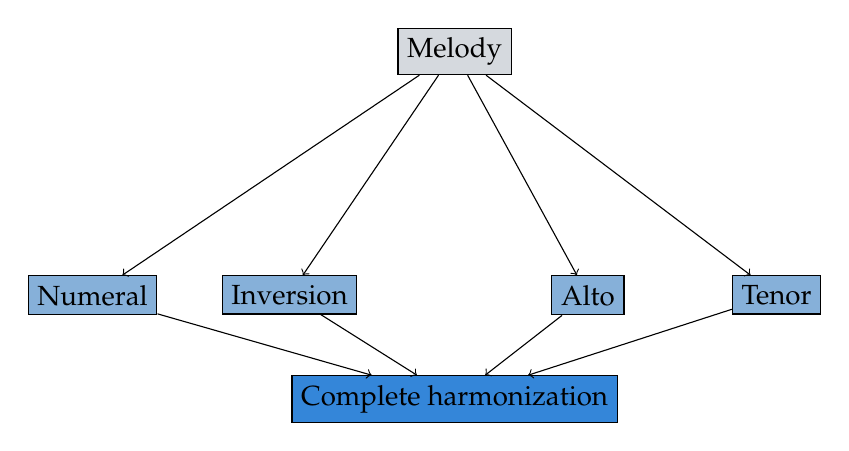
\begin{tikzpicture}
  [
    grow                    = down,
    sibling distance        = 6em,
    level distance          = 4em,
    edge from parent/.style = {draw, -latex}
  ]
  \begin{scope}[init/.style={rectangle,draw,fill=gray},
  			subtask/.style={rectangle,draw,fill=lightblue},
  			goal/.style={rectangle,draw,fill=deepblue}, node distance=1in]
  \node [init] (mel) {Melody};
  \node [goal] (el) [below=1.5in of mel] {Complete harmonization};
  \node [subtask] (a) [below left=1in and 1.2in of mel] {Numeral} edge [->] (el);
  \node [subtask] (b) [below left=1in and 0.2in of mel]{Inversion} edge [->] (el);
  \node [subtask] (c) [below right=1in and 0.5 of mel] {Alto} edge [->] (el);
  \node [subtask] (d) [below right=1in and 1.1in of mel] {Tenor} edge [->] (el);
  \path[->] (mel) edge node {} (a);
  \path[->] (mel) edge node {} (b);
  \path[->] (mel) edge node {} (c);
  \path[->] (mel) edge node {} (d);
  \end{scope}
\end{tikzpicture}
\end{center}
\end{figure}

\section{Methods}

\subsection{Resources}

We gathered the chorales in MusicXML format through the \textsc{music21} \texttt{corpus} module, and which were originally obtained from \citet{greentree2005}. \textsc{music21} is a toolkit for computational musicology maintained by Professor Michael Scott Cuthbert at MIT \citep{cuthbertmusic21} that was used extensively in this thesis. The \textsc{music21} library is built upon a comprehensive array of objects and methods that represent the fundamental musical components introduced in Chapter 1, such as keys and scales. For our purposes, \textsc{music21} was used extensively to transform musical scores into symbolic representations and extract musical features from those scores for machine learning. The library was also used to generate realizations of predicted chorale harmonizations as actual scores, which are provided at the end of Chapter 3. \\

In order to construct and train neural networks, the scientific computing framework Torch was used, which is written in the Lua programming language. The \texttt{rnn} library, which is designed to extend the capabilities of the \texttt{nn} module in Torch, was used to implement recurrent neural networks like RNNs and LSTM networks \citep{leonard2015rnn}. Non-neural models were selected from the fully implemented classification algorithms in the machine learning library \texttt{scikit-learn} \citep{scikit-learn}.

\subsection{Data}

The dataset consists of 326 4-voice chorales gathered from the \textsc{music21} library. Once collected, some manual cleaning was then performed to correct mistakes in the musicXML format related to key signatures and significant mistakes in notation (based on a visual comparison with the Riemenschneider edition of the Chorales). Chorales with significant periods of rest were removed from the dataset because 3-voice harmonies have ambiguous implications in the 4-voice model that the chorales conventionally observe. Next, the chorales were "quantized" to create strictly chordal progressions of 4-voice harmony. Like modern church hymns, Bach's chorales are uniformly structured as chordal progressions, with a consistent beat-long rate of harmonic transition. Therefore, the process of quantizing each chorale into a series of discrete and uniform time steps, each the length of a beat, could be accomplished without damaging the underlying harmonic progression. Eighth notes were removed from the voices to eliminate additional rhythmic complexity. Eighth notes facilitate voice leading in Bach's harmonizations, but rarely function as an essential part of the harmony, making their removal a reasonable design decision. This process of quantizing the chorale into quarter-note samples has been found to be effective in several other studies (\cite{hild1992harmonet}; \cite{madsen2002}; \cite{kaliakatsos2014}). \\

From the chorales, data for each subtask needed to be extracted for each time step of each chorale. For the harmonic analysis subtasks, Roman numeral analysis was implemented to extract the correct Roman numeral and inversion. We relied on a combination of \textsc{music21}'s \texttt{roman} module for initial analysis followed by substantial manual correction due to incomplete functionality in the \texttt{roman} module. The alto and tenor voices were extracted as a sequences of notes encoded as MIDI values. \\

For each time step, a feature vector $\boldx$ was extracted that represents an observation about the melody note. A Python script was then used to preprocess the chorales to extract the above features from each time step of each chorale, and stores the generated training and test data in an HDF5 file. The selected attributes of each feature vector are enumerated below:

\begin{enumerate}
\item The number of sharps in the key signature. Flats were given negative values.
\item The mode (i.e. major or minor) of the chorale.
\item The time signature of the chorale.
\item Beat strength, or metrical accent. A 4/4 measure would be assigned the following pattern: [ 1.0, 0.25, 0.5, 0.25 ]
\item The presence of a fermata - a binary attribute indicating a cadence.
\item Number of beats until the next fermata.
\item Number of measures until the end of the chorale.
\item The melody pitch, encoded as a MIDI value. A search across all chorales indicated that each voice had a well-defined pitch range, verified by \citet{madsen2002}: 
\begin{itemize}
\item \textit{soprano}: [60, 81]
\item \textit{alto}: [53, 74]
\item \textit{tenor}: [48, 69]
\item \textit{bass}: [36, 64]
\end{itemize}
\item The interval to the previous melody note.
\item The interval to the next melody note.
\item The Roman numeral for the previous time step.
\item The inversion for the previous time step.
\end{enumerate}

The first 10 attributes are used for all experiments in Chapter 2, while the final two attributes are introduced only for the "Oracle experiments" in Chapter 3. In the GCT implementation, the two Oracle attributes are substituted for attributes that describes the GCT encoding (root, base, inversion) for the previous time step. \\

These attributes were carefully chosen. The key signature (attributes 1 and 2) and time signature (3) are constant across all features vector for a chorale since they denote chorale-wide features. The pitch of the melody note (8) and the presence of a fermata (5)  provide information about the melody note, but all of the remaining features denote contextual information. Beat strength (4) denotes the melody note's position (and the weight of that position) within the measure. Features 6 and 7 describes the melody's note location with the current phrase. Features 9 and 10 describe the local direction of the melody voice.

\section{Results}
Results for baseline model performance on the Roman numeral analysis subtasks and harmonic prediction subtasks are shown in Table 1. Table 2 lists the frequencies of the most frequent class for each subtask (Table 2), which serves as a basic metric of comparison. With the exception of inversion, all baseline models performed significantly above the most common class frequency. The models performed only marginally better than the MCCF threshold for the inversion subtasks, but the uniquely high MCCF should be taken into account. Amongst the baseline models, the random forest classifier outperformed the other models by a non-trivial degree, averaging 9.75\% increase in accuracy over multinomial logistic regression. 

\begin{table}[h]
\begin{center}
\caption[Table caption text]{\textbf{Baseline model accuracy on test set, harmonization subtasks.}}
\begin{tabular}{l | c c c c}
Classifier & Numeral & Inversion & Alto & Tenor \\ \hline
Multi-Class Logistic & 31.61\% & 59.76\% & 37.55\% & 37.86\% \\
Multinomial Naive Bayes & 27.44\% & 56.66\% & 35.06\% & 34.40\% \\
Random Forests & 49.29\% & 61.64\% & 49.44\% & 45.43\% \\
\end{tabular}
\end{center}
\end{table}

\begin{table}[h]
\begin{center}
\caption[Table caption text]{\textbf{Most common class frequency (MCCF).}}
\begin{tabular}{l | c c}
Subtask & Training Set & Test Set \\ \hline
Numeral & 19.2\% & 19.2\% \\
Inversion & 55.5\% & 57.6\% \\
Alto & 15.7\% & 14.6\% \\
Tenor & 15.6\% & 15.5\%
\end{tabular}
\end{center}
\end{table}

These experiments were repeated after substituting the Roman numeral analysis subtasks with the GCT ones. For the harmonic analysis subtasks, the objective was to now independently predict the root, the harmonic function (base), and the inversion. In this set of experiments, inversion was encoded using the GCT representation, which explains the change in class distribution. The harmonic prediction subtasks, however, remained the same, but are still included in the results shown in Table 2.3. \\

\begin{table}[h]
\begin{center}
\caption[Table caption text]{\textbf{Baseline model accuracy with GCT harmonic analysis subtasks.}}
\begin{tabular}{l c c c c c}
Classifier & Root & Base & Inversion & Alto & Tenor \\ \hline
Multi-Class Logistic & 58.29\% & 56.09\% & 67.06\% & 37.55\% & 37.86\% \\
Multinomial Naive Bayes & 48.19\% & 50.43\% & 62.66\% & 35.06\% & 34.40\% \\
Random Forests & 63.71\% & 59.72\% & 69.73\% & 49.44\% & 45.43\% \\
\end{tabular}
\end{center}
\end{table}

\begin{table}[h]
\begin{center}
\caption[Table caption text]{\textbf{MCCF with GCT subtasks.}}
\begin{tabular}{l | c c}
Subtask & Training Set & Test Set \\ \hline
Root & 28.5\% & 28.0\% \\
Base & 49.5\% & 49.9\% \\
Inversion & 63.9\% & 65.5\% \\
Alto & 15.7\% & 14.6\% \\
Tenor & 15.6\% & 15.5\%
\end{tabular}
\end{center}
\end{table}

\begin{figure*}[ht]
\caption{Baseline model comparison for harmonization subtasks}
\centerline{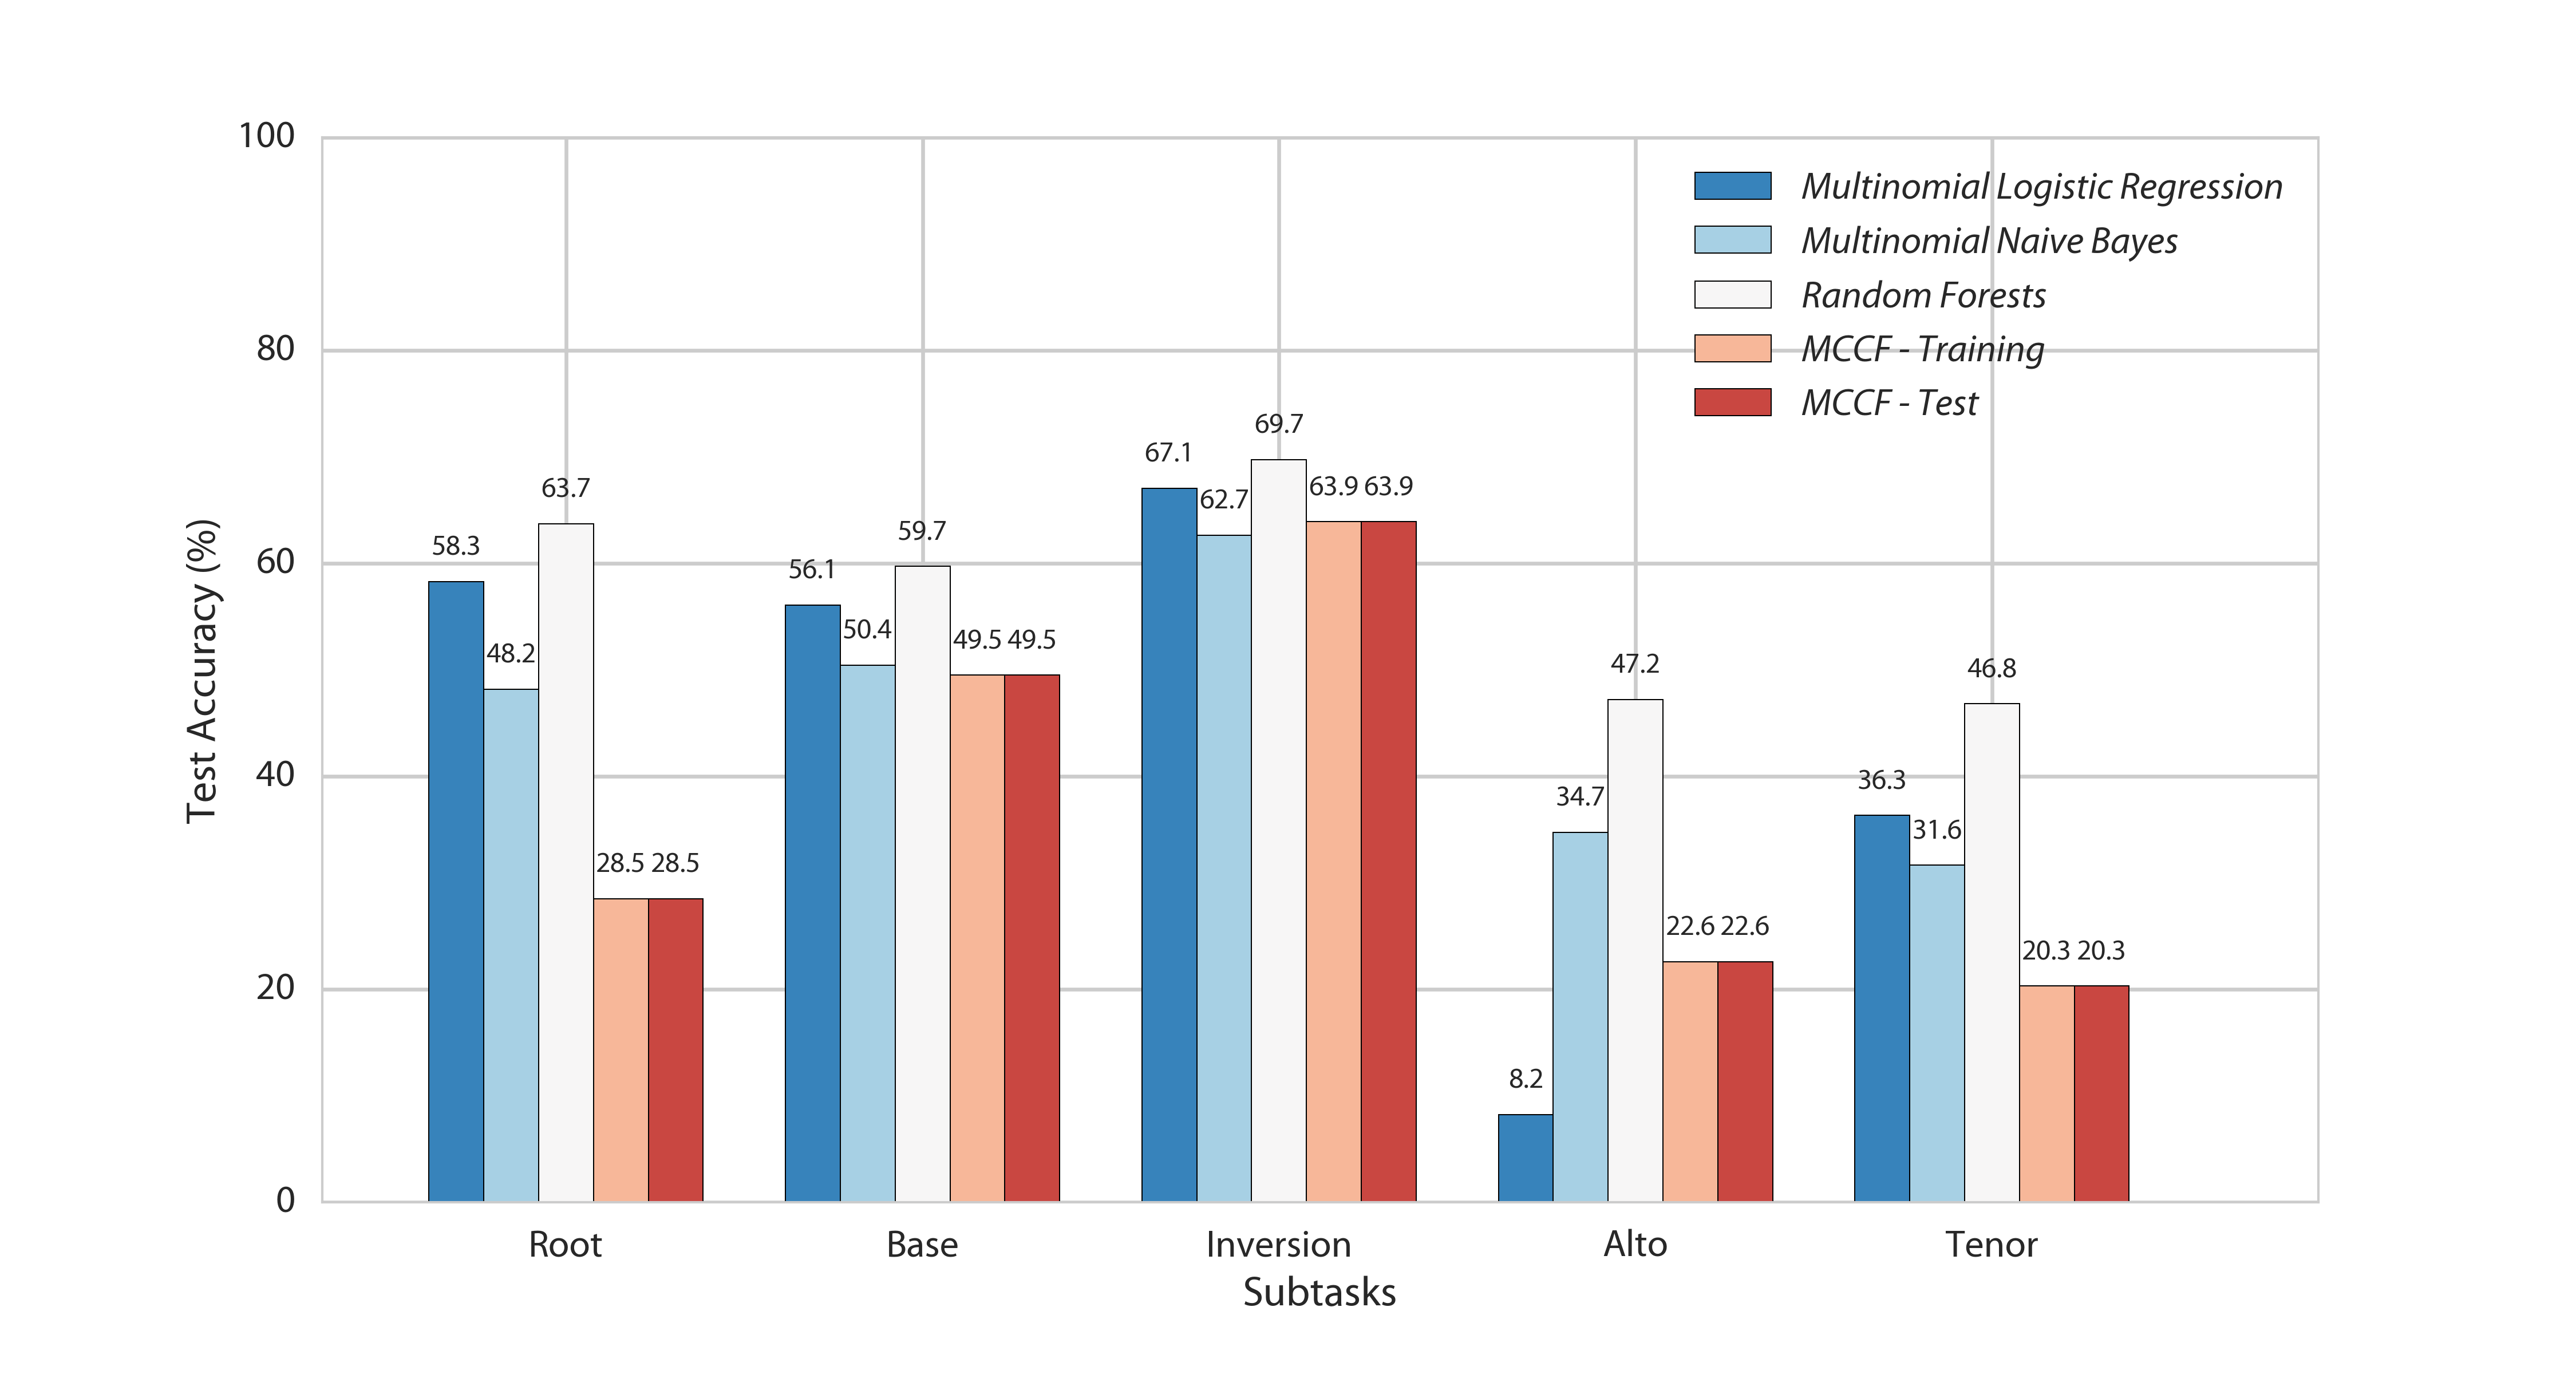
\includegraphics[scale=0.5]{images/subtasks}}
\end{figure*}

\section{Discussion}

Figure 3 provides a visual comparison of baseline model performance across all harmonization subtasks. For all subtasks, a majority of the multinomial models outperformed the MCCF baselines. In particular, Random Forests consistently outperformed the other models, with a 35\% increase in accuracy over the MCCF baseline for the root subtask. However, the multinomial models struggled to perform above the MCCF baselines  for both the base and inversion subtasks, which appears correlated with a high predominance of a single class in the dataset. Musically, this is not surprising. The predominance of a single class in the base subtask is consistent with the frequencies of the major triad found by \citet{cross2008} in the Chorales, while the vast majority of harmonies in the dataset - and in other corpora from the Baroque era - are in root position. In contrast, the more even class distribution of the Roman numeral and GCT root subtasks are consistent with the well-known harmonic complexity of the Chorales. \\

The variation in performance between subtasks suggests a general issue with imbalanced class distributions in the data. Of the 133 output classes for the GCT base subtask, the most common class is associated with 50\% of all observations in entire dataset (this happens to be the major triad), and the top 3 most frequent classes account for 77\% of all observations. Consequently, the vast majority of output classes are observed too infrequently in the training data to be classified accurately in the test data. Imbalanced data is a widely recognized phenomenon in data mining that is comprehensively detailed in \citet{sun2009classification}. The significant advantage achieved using random forests can potentially be explained by its known effectiveness at classification when one or more observations is not sufficient to generally distinguish a class \citep[pg.~18]{breiman2001}.


%%%%%%%%%%%%%
% CHAPTER 3
%%%%%%%%%%%%%

\chapter{Neural models for harmonic analysis and prediction}

\section{Introducing neural networks}

I will now shift focus to supervised learning of the chorales using both non-recurrent and recurrent neural models, seeking to improve upon the baseline models presented in Chapter 2. Neural networks are able to engage in sophisticated decision-making by passing the input forward through the network and making more complex and abstract decisions in the hidden perceptron layers. As demonstrated in the literature review at the beginning of Chapter 2, neural networks are popular in computational musicology for their ability to perform highly complex pattern recognition over large datasets and generalize when given unexpected musical sequences. In particular, recurrent neural networks (RNNs) show great promise in sequence labelling because of their ability to incorporate contextual information about previous computations. In the case of next-step harmonic prediction, we discuss in Chapter 1 the constraints placed on the next harmony by the preceding harmonies. A satisfying harmonic sequence is additionally constrained by the ultimate goal of reaching resolution, and each harmony in the sequence can be labeled as a step towards or away from that goal. Therefore, I hypothesize that a next-step prediction model will benefit from additional features that denote the harmony chosen at the previous time step. This hypothesis will be evaluated by use of an "Oracle experiment."

\section{Methods}

\subsection{Two approaches to harmonization}

The experiments described in this chapter explore harmonization via two different methods. The first approach is predicting harmonization as a series of individual subtasks - identical to the approach in Chapter 2. Collection, a set of the predictions for all subtasks describe the harmony and its voicing for a given time step. The prediction of each subtask, moreover, is independent of the predictions for other subtasks at the same time step. Note that this does not particularly reflect the compositional process of a musician. The choice of inversion in Roman numeral analysis, for example, is dependent upon the chosen Roman numeral, and the selection of pitches for inner voices is dependent on the general harmony intended for that time step. The second approach groups a full set of predictions for all subtasks as a single prediction. This is referred to as the \textit{full harmonization} task, since the harmony and its voicing is decided by a single prediction. The set of output classes consists of all full sets of predictions observed in the training data, where each set of predictions is mapped to a single class, which describes a complete "harmonization". A single harmonization class might represent the following, for instance: D chord, major triad, root position, the 3rd above D in the alto, the 5th above in the tenor. This new approach adds a weak dependency between the subtasks because they are predicted collectively rather than separately. \\

In the full harmonization approach, approximately 5\% of harmonization classes in the test set do not occur in the training set. While this 5\% of classes represents a relatively infrequent set of harmonizations, the neural models will never predict these classes when evaluating test data. To understand why, imagine a model that accepts an image and classifies the content of the image as either a cat, a dog, or a bird. If the model is only shown cats and dog during training time, then it will update its parameters to reflect these observations - namely, that the input image is never of a bird but only either a cat or a dog. Consequently, an image of a bird in the test set will inevitably be misclassified. The images of bird are analogous to these infrequent harmonizations, which will essentially never be predicted. While we do not believe this classification discrepancy significantly affects the results achieved with the full harmonization approach, a better method for encoding harmony in future studies could eliminate this. 

\subsection{Oracle experiment}

Before incorporating recurrent models, I wanted to know if having the context of previous harmonies would in fact improve the model's ability to predict subsequent harmonies. In the field of natural language processing, an Oracle experiment refers to the inclusion to the addition of an "Oracle" in the data that always provides accurate information about some feature. By comparing the original model with the enhanced model, one can directly attribute the difference in error to the absence of the Oracle data. We use this experiment for the full harmonization task by including the correct harmonization class for the previous time step in each input vector. An improvement in performance with the Oracle data suggests that the harmonic information is a valuable component of the input data, and therefore a recurrent model that receives feedback from previous time steps will likely perform well.\\

Attributes 11 and 12 of the feature vector described in section 2.4.2 describe predictions for the harmonic analysis subtasks at the previous time step. Once GCT encoding was introduced, this became 3 features that described the root, base, and inversion of the previous harmony. By providing these features in the input vector, we simulate the feedback provided in a recurrent model from the computation at the previous time step. The baseline models and the "vanilla" neural network were re-evaluated using the Oracle features, using the same training-test split as before.

\subsection{Architecture for neural models}

All neural models were implemented in Torch, using the \texttt{rnn} module for the recurrent components. The "vanilla" neural network (NN) contained 3 layers, with one layer of varying sizes that was optimized based on performance over a validation set. The validation set consisted of 33 chorales randomly extracted from the training set. A lookup table was added as a layer of convolution that takes the input as a vector of indexed features and outputs a matrix where each column represents an embedding for a feature in the original input. After passing through the hidden layer, the intermediate output is transformed by a softmax to output a probability distribution over all possible output classes. The criterion used was negative log likelihood (NLL), and the objective is to continue training until NLL converges to a local minimum. All neural models were trained using backpropagation across all time steps of the chorale. Each chorale was padded with padding inputs mapped to a padding class in order to make each chorale a sequence a length equal to the length of the longest chorale. Optimal learning rates, based on performance over the validation set, varied from 0.01 to 0.001. \\

After noting the success of the Oracle experiment, two recurrent models were constructed with the objective of improving accuracy by feeding in the chorales as a \textit{sequence} of inputs. As discussed in Chapter 1, RNNs include recurrent connections that allow for feedback from the computation that occured at the previous time step. During the forward pass, at each time step in the data sequence, the RNN input layer receives an external input from the $i$th sequence $x^{(i)}_t$ as well as internal feedback from the hidden layer $h_{t}$, and then outputs a distribution $x_{t+1}$ for the next time step. Here, each element of the sequence is a feature vector describing a single melody note, drawn from the same dataset used for previous models. Internally, the network stores $h_t$ as a "memory" of the melody features at time $t + 1$, which will be used to predict the harmonization $x_{t+2}$, and so forth.

\begin{center}
\begin{tikzpicture}
  \matrix (m) [matrix of math nodes,row sep=3em,column sep=4em,minimum width=2em]
  {
     time \to & h_t & \to\\ 
     x^{(i)}_t & R & h_{t+1}\\
     \to & h_{t+1} \text{ (feedback)} & \to\\};
  \path[-stealth]
    (m-1-2) edge (m-2-2)
    (m-2-1.east|-m-2-2) edge [double] (m-2-2)
    (m-2-2.east|-m-2-3) edge [double] (m-2-3)
    (m-2-2) edge (m-3-2);
\end{tikzpicture}
\end{center}

The recurrent layer ($R$) accepts as input a sequence of input vectors describing each time step of a chorale and outputs a corresponding sequence of distributions describing the probability of each harmonization class at each time step. The most likely harmonization for each time step is selected by taking the $\argmax$ of that time step's output distribution, $h_{t+1}$.

$$\argmax h_{t+1} = \argmax_k
\begin{bmatrix} h_{{t+1}_1} \\ h_{{t+1}_2} \\ \vdots \\ h_{{t+1}_k}
 \end{bmatrix}
 $$

The first model is a "simple" recurrent neural network, or S-RNN \citep[p.~56]{goldberg2015nnlp}. The network has a single recurrent hidden layer, The second model is a 5-layer LSTM network with standard input, output, and forget gates. For both models, the hidden layers have a consistent size of 200 neurons. For regularization on the NN and LSTM model, we implemented dropout with probability 0.5 between all hidden-to-hidden layers. Dropout is a technique that address the overfitting problem associated with neural networks by "dropping" a random subset of activations in a given layer of the network. By eliminating a fraction of the signals at each layer, the network becomes comparable to a series of smaller, separately trained networks who outputs are averaged together to obtain a collective prediction.

\section{Results}

First, the "vanilla" neural network (NN) was evaluated on the same individual subtasks used in Chapter 2 for the baseline models, using GCT encoding. Table 3.1 provides the results for the NN performance on each subtasks for both training and test data. The training accuracy and NLL suggest that the neural model did not overfit on the subtasks. And comparing these results to the baseline model results shown in Figure 2.3, the neural network performs on average at the same accuracy rate as Random Forest, the strongest baseline model.

\begin{table}[h]
\begin{center}
\caption[Table caption text]{\textbf{"Vanilla" neural network performance.}}
\begin{tabular}{l *{5}{c}}
Task & Training NLL & Acc\% & Test NLL & Acc\% & Test MCCF \\ \hline
Root & 0.768 & 71.92\% & 1.164 & 58.66\% & 27.7\% \\
Base & 1.265 & 62.48\% & 1.694 & 55.09\% & 48.4\% \\
Inversion & 0.701 & 70.78\% & 0.770 & 67.86\% & 64.5\% \\
Alto & 0.903 & 67.90\% & 1.680 & 42.32\% & 21.7\% \\
Tenor & 0.900 & 67.57\% & 1.721 & 42.66\% & 20.7\%
\end{tabular}
\end{center}
\end{table}

The Oracle experiment demonstrated favorable results and improved performances across the board by a few percentage points. Interestingly, the neural network performs only slightly better than logistic regression on harmonic analysis subtasks, but performs an average of 12.5\% better on prediction of inner voices. \\

\begin{table}[h]
\begin{center}
\caption[Table caption text]{\textbf{Baseline and neural model test accuracy, Oracle experiment. }}
\begin{tabular}{l *{5}{c}}
Classifier & Root & Base & Inversion & Alto & Tenor \\ \hline
Multi-Class Logistic & 59.75\% & 56.49\% & 64.43\% & 38.99\% & 38.93\% \\
Multinomial Na{\"i}ve Bayes & 54.31\% & 48.48\% & 63.06\% & 37.08\% & 34.10\% \\
Random Forests & 71.62\% & 65.85\% & 74.56\% & 53.91\% & 52.20\% \\ \hline
"Vanilla" Network (NN) & 60.86\% & 57.83\% & 69.67\% & 56.27\% & 46.67\%
\end{tabular}
\end{center}
\end{table}

Based on the favorable results from the Oracle experiment, the two recurrent models were constructed and evaluated. Na{\"i}ve Bayes was left out because it consistently underperformed in comparison to the other neural and non-neural models. The recurrent models took significantly longer to training, averaging between 18-24 hours. Random Forest, in contrast, reached convergence in 2-3 minutes. 

\begin{table}[h]
\begin{center}
\caption[Table caption text]{\textbf{Neural and baseline model accuracy, full harmonization task}}
\begin{tabular}{l c c c }
Model & Train NLL & Train & Test \\ \hline
Multinomial Logistic & -- & 42.74\% & 25.15\% \\
Random Forest & -- & 88.41\% & 30.38\% \\ \hline
NN & 1.127 & 67.41\% & 25.59\% \\
S-RNN & 0.756 & 45.95\% & 24.73\% \\
LSTM & 0.807 & 38.01\% & 29.35\%
\end{tabular}
\end{center}
\end{table}

Given that the MFFC frequency is 5\%, these results reveal a promising ability to predict full harmonizations over a large set of harmonization classes ($K = 1980$). Surprisingly though, the recurrent models did not outperform Random Forest.


%%%%%%%%%%

\section{Discussion}

\subsection{Neural network results}

Neural networks proved capable learners for both harmonic analysis and prediction tasks. They outperformed the majority of baseline models and more than doubled accuracy when compared to the MCCF baselines for subtasks with more even class distributions (i.e. lower MCCF), such as the root and the alto and tenor voices. As discussed in Chapter 2, the uneven distribution of output classes means that the model's parameters will be updated predominantly to reflect the most frequent output classes at the expense of learning to recognize the rarer ones. This appears to be the case with the base and inversion tasks, where the network struggled to outperform the fairly high baseline set by the MCCF model. However, the overall performance of the standard neural network is considered a success considering the complexity of these musical tasks. \\

With respect to the recurrent neural models, it was surprising to see them outperformed by the Random Forest baseline model. This may be due to a variety of reasons, including a structural issue in the data or a class imbalance. Yet viewed another way, the Random Forest model performed exceedingly well considering that it does not receive the temporal feedback built into the recurrent models. We hypothesize that the Random Forest model likely generalized well despite the high frequency of a small set of harmonizations - a set mostly consisting of various tonic and dominant triad voicings. The non-recurrent models also benefitted greatly from the context already present in the input feature vector, which informs of the model of the position of the harmony within the measure and within the phrase. Hopefully, more work is done to examine the ability of both the Random Forest model and LSTM networks to perform other predictive musical tasks, and to examine how different features affect the model's sense of context within a musical phrase. 

\subsection{Analyzing Random Forest harmonizations}

Figures 3.1 and 3.2 compare Bach's harmonizations against predicted harmonizations generated by the Random Forest model for the full harmonization task. Note that the "Original" score represents the Bach's score after the quantization process (Section 2.5), and the accuracy rating refers to the average accuracy of harmonization class prediction, where each class describes a set of predictions over all subtasks. While the accuracy over test chorales varied greatly, two chorales were chosen to demonstrate the Random Forest harmonizations in both major and minor with accuracy levels close to the mean (30.38\%). The diagrams were created by reversing the feature extraction process, decoding feature indices and converting them back into musical symbols. The scores were generated using a Python script that used \textsc{music21} to reconstruct the chorale melody and harmonization from the harmonization classes. Minor manual correction was then required to adjust the ranges of inner voices to the proper octave. \\

These figures are clear evidence of the success of this model. The example harmonizations indicate a diversity of harmonic choices and voice-leading patterns. Most cadences are well-executed and provide a satisfying resolution to either tonic or dominant harmonies. In \textit{Helft mir Gotts G{\"u}te preisen} (Figure 3.1), two cadences in particular deserve note. Measure 12 features an authentic cadence to G major ($\flat$\rom{7}), despite no prior introduction of an F$\sharp$ in the soprano voice or other indication of this tonicization. The final measure, moreover, is correctly predicted as a Picardy cadence, resolving to an A major harmony in an A minor key. \\

The ends of phrases were also correctly identified, and the model typically output the same harmony for multiple beats when a fermata was being held. Examining other chorales, the model appears to struggle with more advanced harmonic progressions, particularly where tonicizations occur based on a tonic that is non-diatonic within the original key. Yet on the whole, we have produced harmonizations that largely satisfy the major counterpoint constraints while also reflecting many of the key features in the compositional style of the Chorales.

\subsection{Methods for an improved sequential subtask model}

Recall that the full harmonization task combines an independent series of subtasks into a single prediction task, where each harmonization class represents a set of predictions for the subtasks which are weakly interdependent. There are two significant flaws to this approach. First, the accuracy metric here is harsh because by combining a series of decisions into a single class, a much more fine-grained decision must be made to choose the correct class. This concern could be resolved by creating a more sophisticated accuracy metric that took into account its overall accuracy across all subtasks. The metric should weigh each subtask differently in order to reflect the different levels of musical importance associated with these harmonic aspects. The inversion, for example, is a much less decisive aspect of the harmony than the root or base. The selection of inner voices should also be weighed appropriately to reflect its role as expressing the harmony rather than deciding it. The alto and tenor voices can be often be assigned several different pairs of pitches that express the chosen harmony in a satisfying way. The second issue is that neither approach discussed in Section 3.2 recognizes the highly dependent nature of the subtasks. A \textit{sequential} subtask model may likely improve the results by recognizing the sequential nature of the tasks performed when harmonizing chorales. In particular, predictions for harmonic analysis subtasks would seem a highly useful source of information for predicting the inner voices. The choice of harmony constrains the possibilities of the inner voices since they must support that harmony. So while the current model only provides the melody-focused feature vector for each subtask, a stronger model will consider predictions made for previous subtasks at the same time step. Figure 3.1 shows the proposed ordering of those subtasks.

\begin{figure}[h]
\begin{center}
\caption{Proposed model: sequential prediction of harmonization subtasks.}
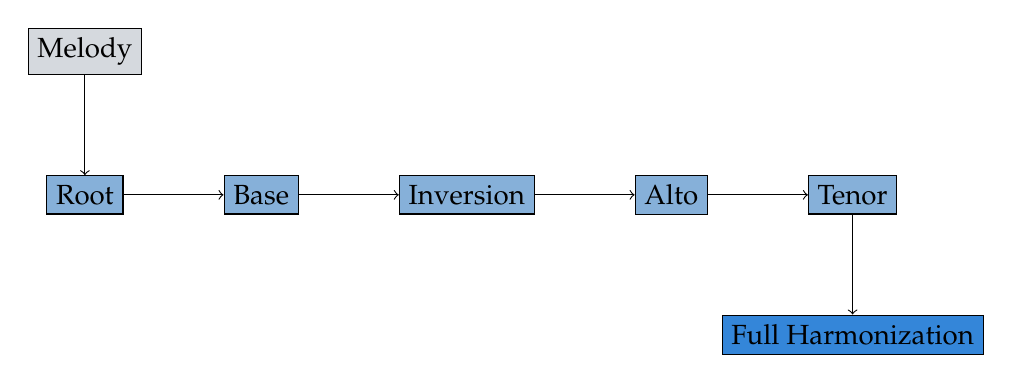
\begin{tikzpicture}
  [
    grow                    = down,
    sibling distance        = 6em,
    level distance          = 4em,
    edge from parent/.style = {latex-latexnew, line width=2pt, arrowhead=4cm}
  ]
  \begin{scope}[start/.style={rectangle,draw,fill=gray},
  			end/.style={rectangle,draw,fill=deepblue},
  			env/.style={rectangle,draw,fill=lightblue}]
  \node [start] (mel) {Melody};
  \node [env] (a) [below=0.5in of mel] {Root};
  \node [env] (b) [right=0.5in of a] {Base};
  \node [env] (c) [right=0.5in of b]{Inversion};
  \node [env] (d) [right=0.5in of c] {Alto};
  \node [env] (e) [right=0.5in of d] {Tenor};
  \node [end] (f) [below=0.5in of e] {Full Harmonization};
  \path[->] (mel) edge node {} (a);
  \path[->] (a) edge node {} (b);
  \path[->] (b) edge node {} (c);
  \path[->] (c) edge node {} (d);
  \path[->] (d) edge node {} (e);
  \path[->] (e) edge node {} (f);
  \end{scope}
\end{tikzpicture}
\end{center}
\end{figure}

We briefly describe this approach mathematically. Assume for the sake of notation that there are only three subtasks. Then the objective is to select
\begin{align}
\argmax_{x, y, z} P(X=x, Y=y, Z=z | \boldX)
\end{align} 

where X, Y, and Z are random variables associated with a specific subtask and can only takes value representing the subtask's output classes. $\boldX$ represents the input data, and let $\hat{x}, \hat{y}, \hat{z}$ be the predicted classes for the 3 subtasks. Then by the chain rule, we can show that
\begin{align}
\hat{x}, \hat{y}, \hat{z} &= \argmax_{x, y, z} P(X=x, Y=y, Z=z | \boldX) \\
				  &= \argmax_{x,y,z} P(X=x | \boldX, Y=y, Z=z) \cdot P(Y=y | \boldX, Z=z) \cdot P(Z=z | \boldX)
\end{align}

While mathematically equivalent, the implementation suggested by Equation 3.3 would consist of separate classifiers for each subtask, where each classifier is trained to predict its respective subtask given the original input vector $\boldx$ along with the predictions for the previous subtasks in the sequence. To reduce the output space represented by all possible set of predictions for all subtasks, the model would only consider sets of predictions that occur in the training set. \clearpage

\fancyhf{}
\fancyhead[C]{\bfseries Figure 3.1}
\fancyhead[R]{\thepage}
\begin{figure}[h]
\caption[Example harmonization: \textit{Helft mir Gotts G{\"u}te preisen}]{Example harmonization of \textit{Helft mir Gotts G{\"u}te preisen}}
\begin{center}
\makebox[\textwidth]{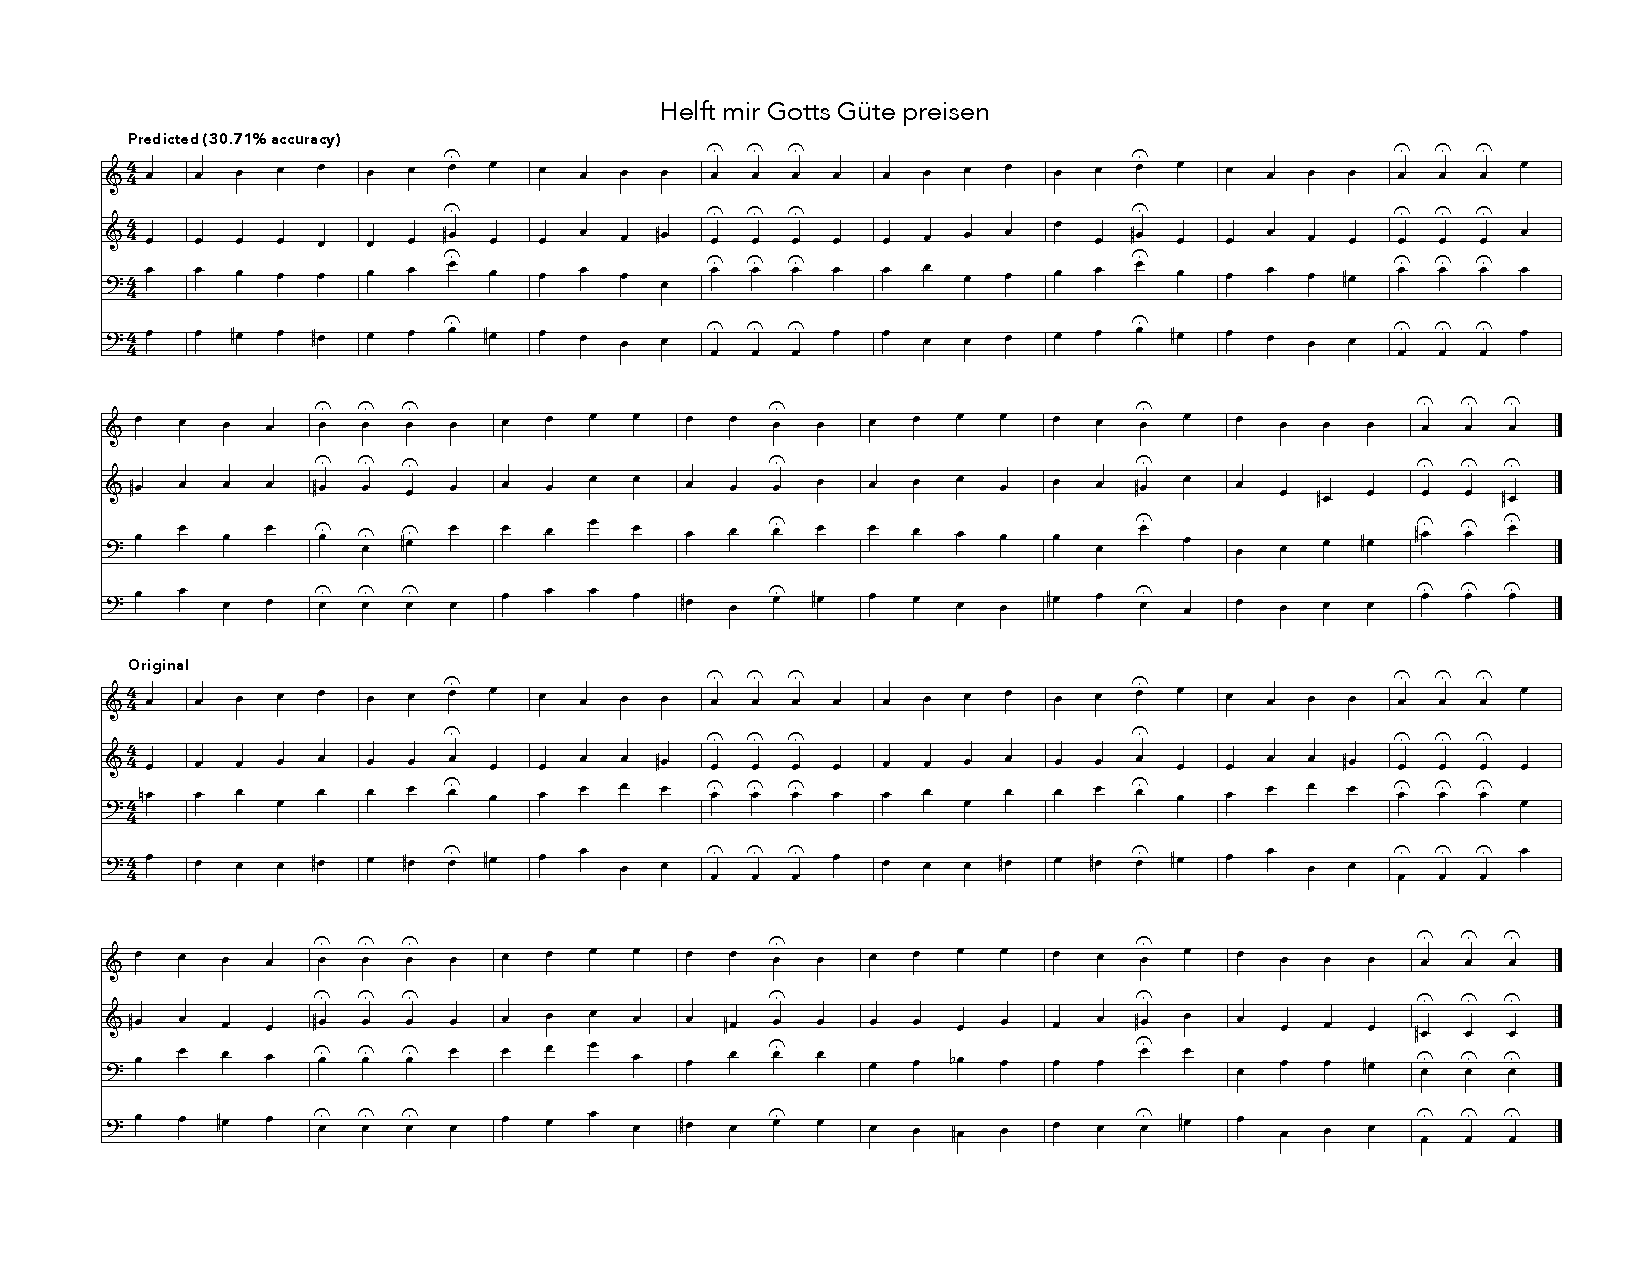
\includegraphics[width=\paperwidth]{examples/ex_minor_1.pdf}}
\end{center}
\end{figure}
\newpage

\fancyhf{}
\fancyhead[C]{\bfseries Figure 3.2}
\fancyhead[R]{\thepage}
\begin{figure}[h]
\caption[Example harmonization: \textit{Herr Jesu Christ, dich zu uns wend}]{Example harmonization of \textit{Herr Jesu Christ, dich zu uns wend}}
\begin{center}
\makebox[\textwidth]{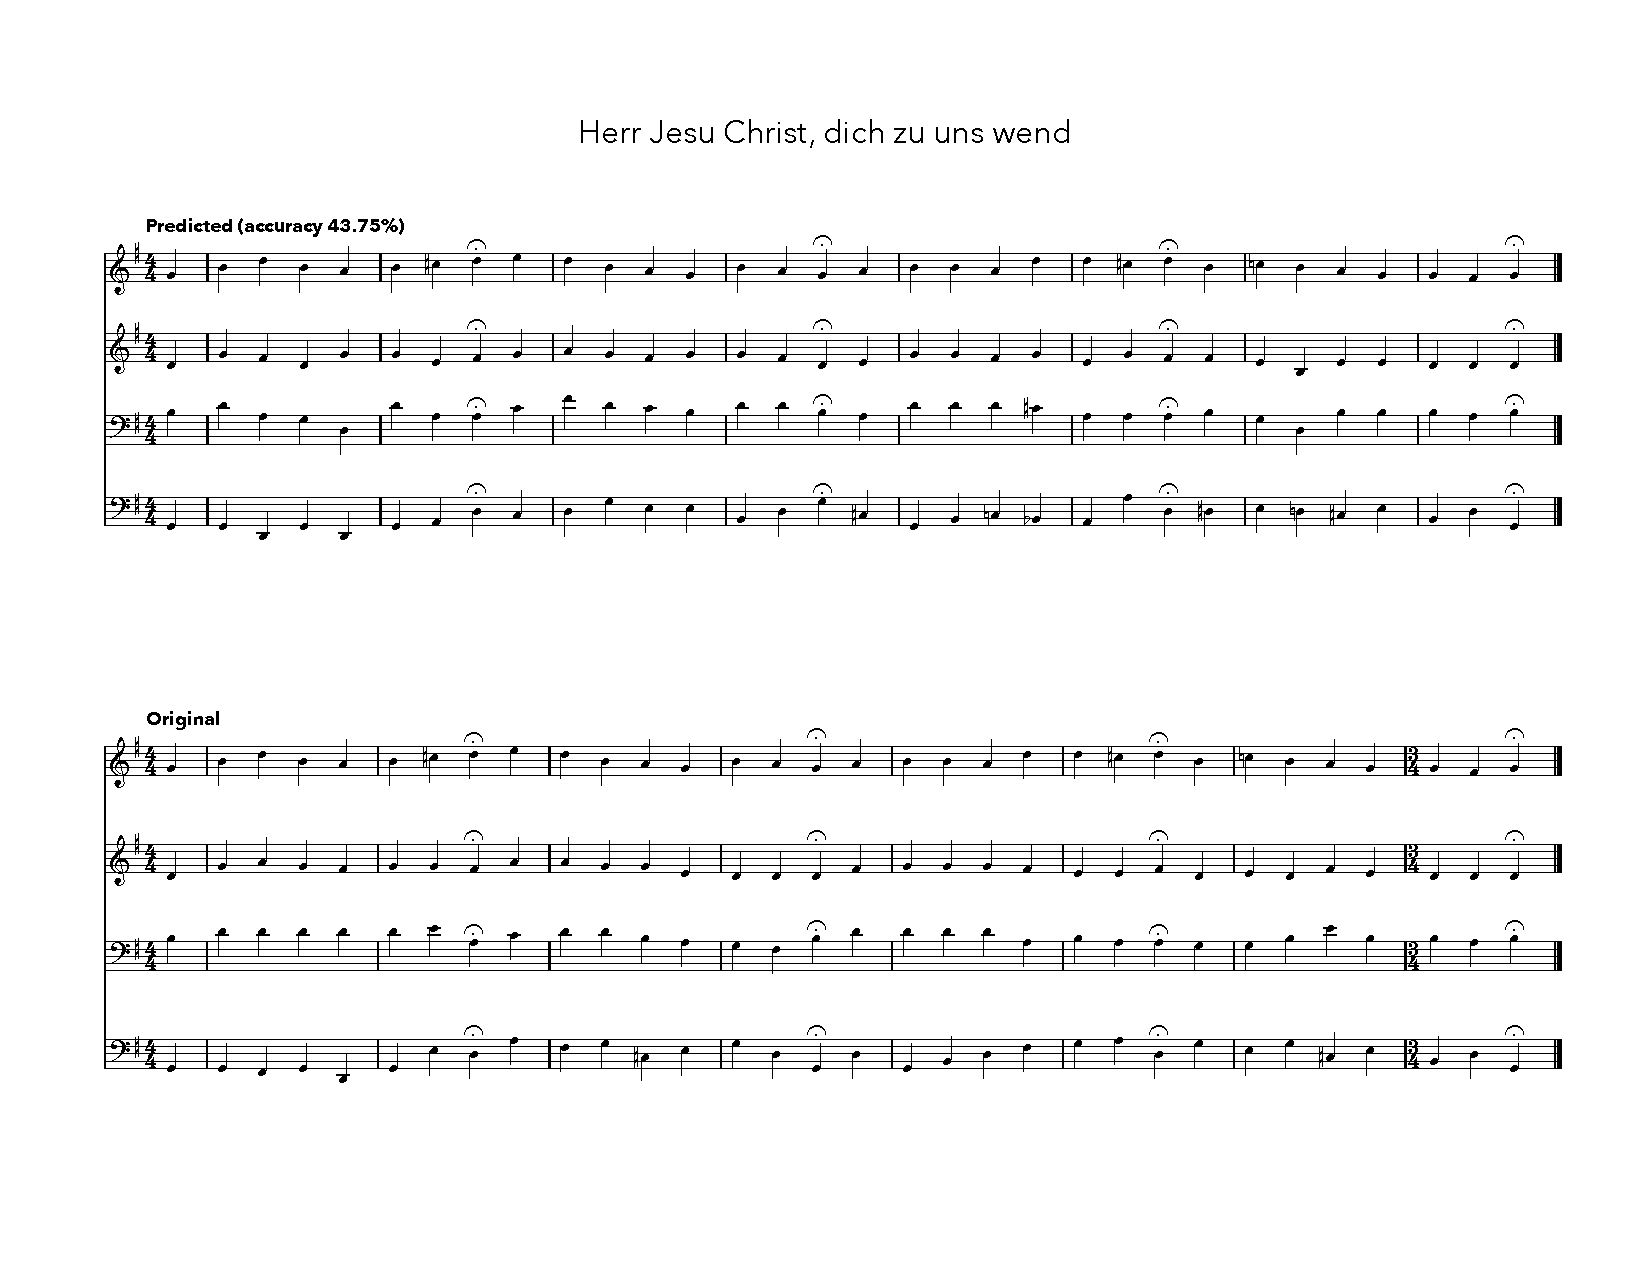
\includegraphics[width=\paperwidth]{examples/ex_major_1.pdf}}
\end{center}
\end{figure}
\fancyhf{}
\fancyhead[R]{\thepage}



%%%%%%%%%%%%
% CHAPTER 4
%%%%%%%%%%%%


\chapter{Further exploration: Bach's Inventions}

\section{Generalizing the harmonization model}

It must be admitted that a model trained to harmonize chorales has limited utility in modern times (although it might have made Bach's work as \textit{Kapellmeister} a bit easier). Musicians today mainly look to Bach's Chorales as early model compositions for 4 voices and for theory-related exercises. Moreover, the Chorales themselves use a limited rhythmic and textural vocabulary, since the rate of harmonic change and many other stylistic properties remain constant. This simplicity makes the chorales advantageous for statistical learning and allows our models to output a uniform set of harmonizations over all inputs. But as chorale harmonization is increasingly well-understood as a computational task, it is worth recognizing the ways in which the chorale harmonization model can be extended to more common musical processes. As one potential application, I will explore the task of composing a counterpoint line given an input melody, and how this might be approached from a computational standpoint. We will refer to this task as \textit{contrapuntal melodic generation} - the composition of a melody in counterpoint with another melody. This task is intentionally open-ended and could be applied to a wide variety of musical corpora. For this chapter, I will focus on how one might potentially implement such a model for Bach's 15 Inventions. Bach's Inventions were selected because they represent exemplary two-voice counterpoint compositions that use Bach's harmonic language, which allows for comparison with the chorale model. Despite being written explicitly as musical exercises, the Inventions are far more melodically and rhythmically complex than the Chorales.

\subsection{Added complexity}
Generating harmonizations for inventions introduces several new layers of musical complexity that were not considered when harmonizing the chorales. One is \textit{rhythmic} complexity, since Invention melodies cannot be effectively quantized into uniform samples as we did with the Chorales, so a method for representing rhythmic features in the contrapuntal melody is need. One method for describing rhythm is to generate predictions at the level of the smallest rhythmic unit in the Invention. For example, if the smallest rhythmic unit in a melody is the 32nd note, then each measure of the melody would be divided into 32 samples. A prediction of the pitch (or a rest) for the contrapuntal melody would be output correspondingly for each sample. Rhythmic variation would then be introduced into the contrapuntal melody by defining the duration of a note or rest as the number of consecutive samples for which the same pitch or rest is predicted by the model. \citet{eck2002blues} found this approach effective for composing blues melodies. An similar but alternative method for describing pitch alongside rhythm was proposed by \citet{franklin2006jazz}, where separate LSTMs are trained to decide pitch and duration. \\

An additional layer of complexity to consider is the need for subject identification. In an Invention, one or more melodic motives govern the development of the entire work, and each motive is restated in various transformations. Collectively, we refer to these motives, or subjects, within the work as the "invention" \citep[p.~10]{dreyfus1996bach}. Dreyfus argues that the composition process behind an Invention is in many ways analogous to process behind writing an oration, which he describes in terms of Ciceronian rhetoric. In the same way that a writer "invents" a speech based on a central idea and then provides arguments and counterarguments, Bach's "obsession with inventive process" led him to centralize his Inventions around the development of a musical subject \citep[p.~35]{dreyfus1996bach}. Therefore, subject identification must be a critical initial stage of analysis before composing a contrapuntal melody. The "invention" of the work reveals the melodic, harmonic, and rhythmic material used in the Invention, and features from the subject should be extracted to create contrapuntal melodies. \\

A final layer of complexity to note is the \textit{form}, or large-scale structure of the Invention. Inventions typically consist of a series of thematic statements interleaved with episodes - modulatory sections that are melodically derived from the subject and create transitions between thematic statements in different keys. Return to the oratory analogy provided by Dreyfus, these sections are the arguments and counterarguments that are presented in between restatements above the main idea. The remaining sections of the Invention are termed "elaborations", which refers to the sections of each piece that connect the larger sections of the piece and do not typically contain thematic states. This includes small cadential phrases that smooth the transitions to a new tonicization, or the codettas that appear at the end of some Inventions. Each type of section has a specific set of conventions that govern its structure as well as the relationship between the two voices.

\subsection{Subject identification}
Bach's Inventions are two-voice compositions, where the lower voice can be characterized as a \textit{function} of the upper voice. In order for the model to learn the harmonic and rhythmic material that Bach employs in the work, the model should first identify and extract features from the Invention's primary \textit{subject}. Identifying the subject generally straightforward for the listener, since the primary subject is typically the first statement in the upper voice. However, inventions can contain multiple subjects with varying levels of importance. And in Invention No. 6 in E major, Bach introduces two subjects of equal importance and develops them both consistently throughout. Therefore, a better approach might be to identify subjects by selecting melodic ideas based on the frequency with which they are restated. \citet{dreyfus1996bach} notes that the frequency of a subject is directly correlated with its importance in the Invention - a principle of repetition that is generally true of melodies in Western music. One candidate algorithm for subject identification based on repetition is hierarchal agglomerative clustering (HAC), which can learn to "cluster" melodic segments based on a supplied distance metric. \citet{nagler2014schubot} applied HAC to the task of motivic analysis in Schubert's song cycle \textit{Die Winterreise} and found promising results in extracting the main motive from each song. However, a significant difficulty in subject identification would be the harmonic and rhythmic transformations that are often applied to the subject when it is restated. For this task, it could be useful to encode the melody as a series of intervals rather than pitches in order to identify subjects in their original form as well as their transformed state. \\

\begin{figure*}[h]
\caption[Invention No. 4 in D Minor (BWV 775), subject and transformations]{ The subject and transformations in Invention No. 4 in D Minor, BWV 775.  }
\centerline{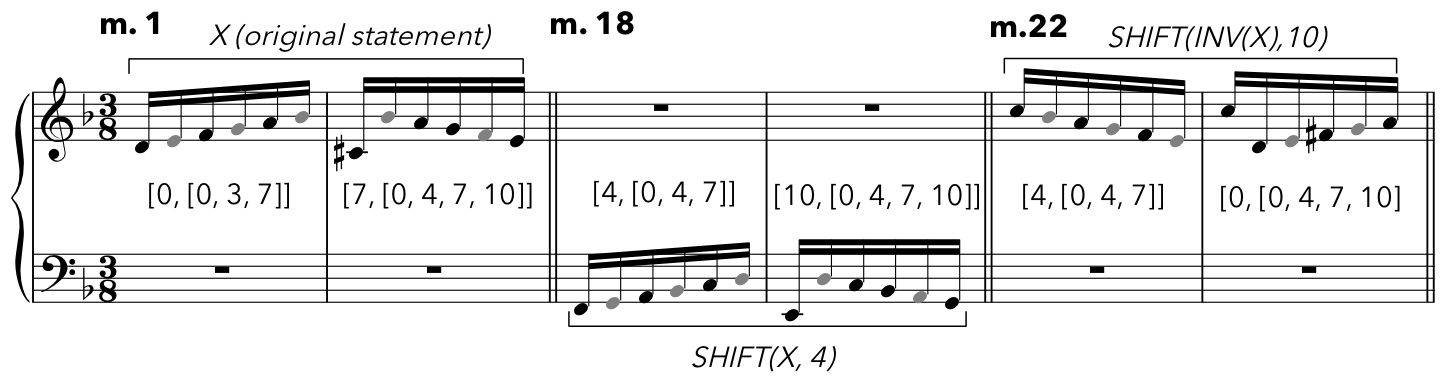
\includegraphics[scale=0.3]{examples/ex1}}
\end{figure*}


\subsection{Form identification}
Once rhythmic and melodic features are extracted from the subject, the model can incorporate these in order to analyze the large-scale structure of the Invention and divide the work into a series of sections. One classifier could be trained to create the general boundaries of each section, while a separate classifier could label each section as a thematic statement ($T$), episodes ($S$), and elaborations ($E$) by analyzing if and how the subject is presented in the upper voice. Complete, sequential statements of the subject suggest a thematic statement, while partial and transformed subject statements will suggest an episode. Elaborations will most likely differentiate themselves by the unique and less repetitiv e melodic material.

\subsection{Harmonic identification}
Before generating the melody, a useful preprocessing step would be to perform harmonic analysis over the upper voice. The classifier would be trained to accept the upper voice as input and output a sequence of corresponding harmonic encodings. This task is well-suited to the model presented in Chapter 2 and 3, where information about a segment of the melody would be classified as a GCT-encoded harmony. While many pleasant melodies can be generated for the counterpoint melody, the most crucial constraint is harmonic agreement. A crucial purpose of the contrapuntal lower voice is to support the upper voice in harmony. The upper voice typically guides the progression, while the lower voice may echo and reinforce harmonic transitions, as Figure 3a illustrates. This relationship reverses when the contrapuntal voice contains a thematic statement, at which point the upper voice may provide harmonic support.  \\

The primary technique for implying harmonies is the one-voice Invention melodies is the use of scalar and triadic passages. Not coincidentally, many of Bach's subjects are constructed to facilitate various transformations (\textit{SHIFT}, \textit{INV}, \textit{AUGMENT}, etc.) and be harmonically indicative. However, given a scalar or triadic passage, it can be difficult to determine which of many potential chords is most strongly implied. There are several important indicators, including the harmony in the previous melodic unit and the beat strength of the notes in the current unit. A recurrent model would likely perform well on this task because of the sequential format of the data (representing the upper voice as a \textit{sequence} of melodic units) and the feedback loop that would provide information about preceding harmonies. The size of each melodic unit, however, is an additional parameter that would require adjustment since the implied harmonies have varying durations (Figure 3b). \\

\begin{figure*}[h]
\caption[Invention No. 13 in A Minor (BWV 784), excerpts]{ Excerpts from Invention No. 13 in A Minor, BWV 784.  }
\centerline{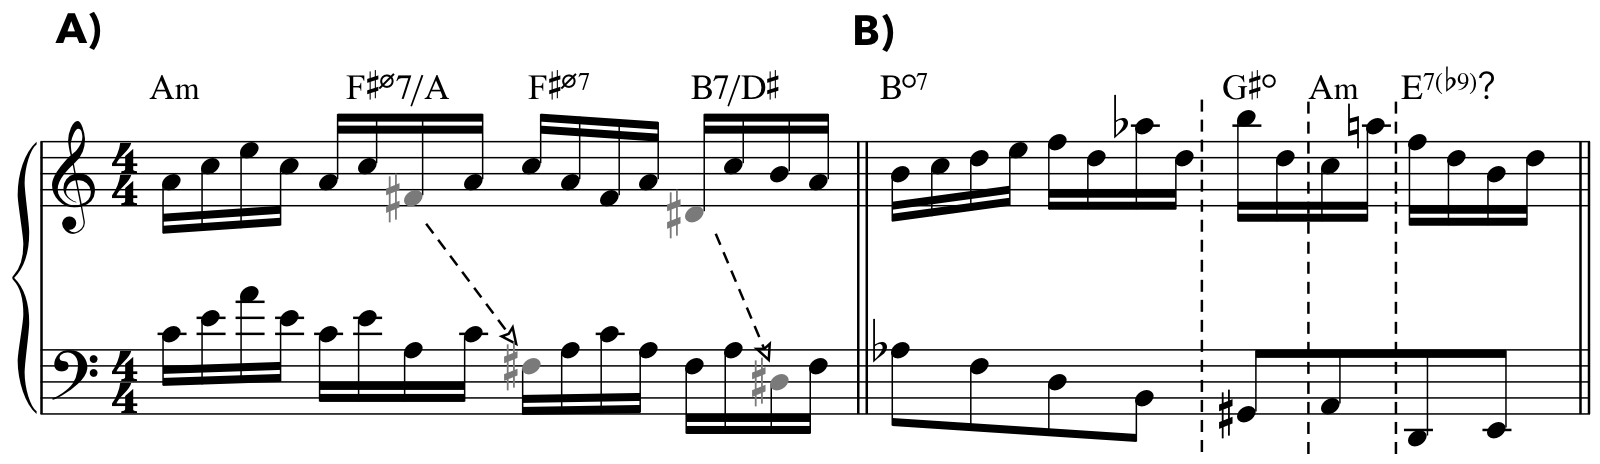
\includegraphics[scale=0.27]{examples/ex2}}
\end{figure*}

\subsection{Contrapuntal melodic generation}
Using the structural information gathered during preprocessing, a final classifier is trained to generate the contrapuntal melody. The classifier would accept input features describing the current relevant subject, the current section of the form, and the current implied harmony, as well as melodic features related to the upper voice near time $t$. The output feature would describe the most likely pitch for time $t$, with an implied duration of the length of the time step. Consecutive time steps of the same pitch could be merged to represented longer notes. \\

The generalization of this model allows for a wide range of corpora to be incorporated into the training data. Stylistically similar candidates include Bach's Sinfonias (the 3-voice equivalent of the Inventions) and the Fugues. Stylistically separate candidates include Palestrina's masses and motets, which feature significant contrapuntal and imitative composition and contain melodic motives that are developed in multiple voices. Incorporating a larger musical dataset during training will improve model performance and generalize the model's musical style. Further work should be done to explore this extension of the harmonization task to various musical corpora.\clearpage

\section{Conclusion}

In this paper, we applied a variety of neural and non-neural models to different musical processes that are components of chorale harmonization. These models are meant to supplement existing work on computational approaches to generative and completive musical tasks. The Random Forest model and recurrent neural models proved to be most effective at learning harmonization tasks, bringing into question what forms of musical context are necessary to produce effective harmonizations. Comparison of predicted Random Forest harmonizations with Bach's "correct" version demonstrates that the model has a promising ability to learn musical structure and connect temporally distant events.

\subsection{Code and related files}

All code and data related to this paper is freely available on GitHub at\\ \url{https://github.com/glasperfan/thesis/}.
\clearpage
\pagestyle{fancy}
\renewcommand{\headrulewidth}{0pt}
\fancyhf{}
\fancyhead[R]{\thepage}
\printbibliography


\end{document}